\documentclass[10pt,a4paper]{article}
\usepackage[margin=18mm,top=22mm,bottom=18mm,headsep=7mm,footskip=9mm]{geometry}
\usepackage{fontspec,amsmath,amssymb,array,tabularx,xcolor,colortbl,tikz,fancyhdr,hyperref}
\usetikzlibrary{arrows.meta}
\setmainfont{NotoSansKR-Regular.ttf}[Path=../../../common/assets/fonts/,BoldFont=NotoSansKR-Semibold.ttf]
\newfontfamily\brandfont{NotoSansKR-Regular.ttf}[Path=../../../common/assets/fonts/,BoldFont=NotoSansKR-Semibold.ttf]
\definecolor{ink}{HTML}{25343D}
\definecolor{accent}{HTML}{216B7A}
\definecolor{muted}{HTML}{637078}
\definecolor{grid}{HTML}{D2DCDF}
\definecolor{soft}{HTML}{F2F6F6}
\definecolor{vectorblue}{HTML}{266CA8}
\definecolor{answerred}{HTML}{C42030}
\newif\ifanswers\answersfalse
\hypersetup{colorlinks=true,urlcolor=accent,pdftitle={OZ Lab AI Study: Sigmoid and Logistic Regression},pdfauthor={OZ Lab}}
\setlength{\parindent}{0pt}\setlength{\parskip}{2pt}\setlength{\headheight}{21pt}
\setlength{\tabcolsep}{4pt}\renewcommand{\arraystretch}{1.08}\arrayrulecolor{grid}
\pagestyle{fancy}\fancyhf{}
\fancyhead[L]{\brandfont\fontsize{8}{10}\selectfont\bfseries\color{ink}OZ Lab\quad AI Study}
\fancyhead[R]{\brandfont\fontsize{7}{10}\selectfont\color{muted}Sigmoid / Logistic Regression}
\fancyfoot[L]{\brandfont\fontsize{6.8}{9}\selectfont\color{muted}DeepLearning.AI / Stanford Online\quad C1 W3\quad SLIDES 106 TO 124}
\fancyfoot[R]{\brandfont\fontsize{8}{10}\selectfont\color{ink}0\thepage\quad{\color{muted}/\ 09}}
\renewcommand{\headrulewidth}{.3pt}
\renewcommand{\headrule}{\hbox to\headwidth{\color{grid}\leaders\hrule height\headrulewidth\hfill}}
\newcommand{\sect}[2]{\par\vspace{2mm}{\brandfont\fontsize{10}{15}\selectfont\bfseries\color{accent}#1}\quad{\fontsize{14}{19}\selectfont\bfseries\color{ink}#2}\par\vspace{3mm}}
\newcommand{\q}[2]{\par\vspace{3mm}\noindent\makebox[7mm][l]{\brandfont\fontsize{9}{14}\selectfont\bfseries\color{accent}#1}\begin{minipage}[t]{\dimexpr\linewidth-7mm}\fontsize{9.3}{14}\selectfont #2\end{minipage}\par\vspace{1mm}}
\newcommand{\note}[1]{\par\hspace*{7mm}\begin{minipage}{\dimexpr\linewidth-7mm}\fontsize{7.5}{10.5}\selectfont\color{muted}* #1\end{minipage}\par}
\newcommand{\formula}[1]{\par\vspace{1mm}\begingroup\setlength{\fboxsep}{2.3mm}\colorbox{soft}{\begin{minipage}{\dimexpr\linewidth-4.6mm}\fontsize{10}{15}\selectfont$\displaystyle #1$\end{minipage}}\endgroup\par\vspace{1mm}}
\newcommand{\given}[1]{\par\vspace{2mm}\hspace*{7mm}{\fontsize{9.3}{14}\selectfont$\displaystyle #1$}\par\vspace{1mm}}
\newcommand{\ansblank}[2]{\makebox[#1]{\strut\ifanswers\smash{\textcolor{answerred}{\ensuremath{#2}}}\else\textcolor{grid}{\rule{#1}{.3pt}}\fi}}
\newcommand{\cellwork}[1]{\smash{\makebox[0pt]{\ifanswers\textcolor{answerred}{\shortstack[c]{#1}}\fi}}}
\newcommand{\tablerow}{\rule[-1.8mm]{0pt}{7mm}}
\newcommand{\solution}[2]{\par\vspace{1.5mm}\begin{minipage}[t][#1][t]{\linewidth}\vspace{0pt}\fontsize{8}{11}\selectfont\ifanswers\leavevmode\color{answerred}#2\else{\color{grid}\hrule height .3pt}\fi\end{minipage}\par}
\newcommand{\pick}[3]{{\leavevmode\ifanswers\ifnum#1=#2\color{answerred}\fi\fi$\square$\ #3}}
\newcommand{\choices}[3]{\par\vspace{1.5mm}\hspace*{7mm}{\fontsize{8.5}{13}\selectfont\pick{1}{#3}{#1}\qquad\pick{2}{#3}{#2}}\par\vspace{1mm}}
\AtBeginDocument{\fontsize{9.3}{14}\selectfont\color{ink}}
\begin{document}
{\brandfont\fontsize{18}{23}\selectfont\bfseries Sigmoid / Logistic Regression\par}
\vspace{1mm}{\fontsize{10.5}{15}\selectfont From numerical predictions to classes and probabilities}\hfill{\ifanswers\color{answerred}\bfseries Worked answers\else\color{muted}Hand-calculation worksheet\fi}\par
\vspace{3mm}{\fontsize{8}{12}\selectfont\color{muted}Name\quad\rule{33mm}{.3pt}\hfill Date\quad\rule{28mm}{.3pt}}\par
\sect{01}{Binary Classification}
\note{Synthetic practice data\quad Sensor signal $x$ predicts status $y$\quad Normal $0$, abnormal $1$}

\q{1}{Write the possible target values and explain the positive class}
\given{y\in\{\ansblank{10mm}{0},\ansblank{10mm}{1}\}\qquad \text{Positive Class}\;y=\ansblank{10mm}{1}}
\solution{8mm}{Positive does not mean a desirable state\quad Here label $1$ indicates an abnormal reading}
\q{2}{Use line A, fitted to the first six examples, to calculate predictions and classes}
\formula{f_A(x)=0.1x-0.1\qquad \hat y=\begin{cases}1& f_A(x)\ge0.5\\0& f_A(x)<0.5\end{cases}}
\begingroup\fontsize{8.3}{11}\selectfont
\begin{tabularx}{\linewidth}{@{}*{5}{>{\centering\arraybackslash}X}@{}}
\rowcolor{soft}\tablerow Sensor $i$ & $x$ & $y$ & $f_A(x)$ & $\hat y$\\\hline
\rule[-2mm]{0pt}{10mm} 1 & $1$ & $0$ & \cellwork{$0.1(1)-0.1$\\$=0.00$} & \cellwork{$0$}\\\hline
\rule[-2mm]{0pt}{10mm} 2 & $2$ & $0$ & \cellwork{$0.1(2)-0.1$\\$=0.10$} & \cellwork{$0$}\\\hline
\rule[-2mm]{0pt}{10mm} 3 & $6$ & $1$ & \cellwork{$0.1(6)-0.1$\\$=0.50$} & \cellwork{$1$}\\\hline
\rule[-2mm]{0pt}{10mm} 4 & $8$ & $0$ & \cellwork{$0.1(8)-0.1$\\$=0.70$} & \cellwork{$1$}\\\hline
\rule[-2mm]{0pt}{10mm} 5 & $9$ & $1$ & \cellwork{$0.1(9)-0.1$\\$=0.80$} & \cellwork{$1$}\\\hline
\rule[-2mm]{0pt}{10mm} 6 & $10$ & $1$ & \cellwork{$0.1(10)-0.1$\\$=0.90$} & \cellwork{$1$}\\\hline
\end{tabularx}\endgroup\par
\q{3}{Plot A\textquotesingle s predictions over the actual data and connect them with a straight line}
\par\noindent\makebox[\linewidth][c]{\begin{tikzpicture}[x=1cm,y=1cm]
\path[use as bounding box] (-.85,-.45) rectangle (15.05,4.95);
\draw[grid,line width=.22pt] (0.00000,0.00000)--(0.00000,4.40000);
\draw[grid,line width=.22pt] (1.45000,0.00000)--(1.45000,4.40000);
\node[below,fill=white,inner sep=.5pt] at (1.45000,0.55000){\scriptsize$1$};
\draw[grid,line width=.22pt] (2.90000,0.00000)--(2.90000,4.40000);
\node[below,fill=white,inner sep=.5pt] at (2.90000,0.55000){\scriptsize$2$};
\draw[grid,line width=.22pt] (4.35000,0.00000)--(4.35000,4.40000);
\node[below,fill=white,inner sep=.5pt] at (4.35000,0.55000){\scriptsize$3$};
\draw[grid,line width=.22pt] (5.80000,0.00000)--(5.80000,4.40000);
\node[below,fill=white,inner sep=.5pt] at (5.80000,0.55000){\scriptsize$4$};
\draw[grid,line width=.22pt] (7.25000,0.00000)--(7.25000,4.40000);
\node[below,fill=white,inner sep=.5pt] at (7.25000,0.55000){\scriptsize$5$};
\draw[grid,line width=.22pt] (8.70000,0.00000)--(8.70000,4.40000);
\node[below,fill=white,inner sep=.5pt] at (8.70000,0.55000){\scriptsize$6$};
\draw[grid,line width=.22pt] (10.15000,0.00000)--(10.15000,4.40000);
\node[below,fill=white,inner sep=.5pt] at (10.15000,0.55000){\scriptsize$7$};
\draw[grid,line width=.22pt] (11.60000,0.00000)--(11.60000,4.40000);
\node[below,fill=white,inner sep=.5pt] at (11.60000,0.55000){\scriptsize$8$};
\draw[grid,line width=.22pt] (13.05000,0.00000)--(13.05000,4.40000);
\node[below,fill=white,inner sep=.5pt] at (13.05000,0.55000){\scriptsize$9$};
\draw[grid,line width=.22pt] (14.50000,0.00000)--(14.50000,4.40000);
\node[below,fill=white,inner sep=.5pt] at (14.50000,0.55000){\scriptsize$10$};
\draw[grid,line width=.22pt] (0.00000,0.00000)--(14.50000,0.00000);
\node[left,fill=white,inner sep=.5pt] at (0.00000,0.00000){\scriptsize$-0.2$};
\draw[grid,line width=.22pt] (0.00000,0.55000)--(14.50000,0.55000);
\node[left,fill=white,inner sep=.5pt] at (0.00000,0.55000){\scriptsize$0$};
\draw[grid,line width=.22pt] (0.00000,1.92500)--(14.50000,1.92500);
\node[left,fill=white,inner sep=.5pt] at (0.00000,1.92500){\scriptsize$0.5$};
\draw[grid,line width=.22pt] (0.00000,3.30000)--(14.50000,3.30000);
\node[left,fill=white,inner sep=.5pt] at (0.00000,3.30000){\scriptsize$1$};
\draw[-{Stealth[length=1.7mm]},ink,line width=.5pt] (0.00000,0.55000)--(14.72,0.55000) node[right]{\scriptsize$x$};
\draw[-{Stealth[length=1.7mm]},ink,line width=.5pt] (0.00000,0.00000)--(0.00000,4.550000000000001) node[above]{\scriptsize$y,\ f_A(x)$};
\draw[muted,dashed,line width=.55pt] (0.00000,1.92500)--(14.50000,1.92500);
\fill[vectorblue] (1.45000,0.55000) circle(1.8pt);
\node[vectorblue,above right,fill=white,inner sep=.7pt] at (1.45000,0.55000){\scriptsize$1$};
\fill[vectorblue] (2.90000,0.55000) circle(1.8pt);
\node[vectorblue,above right,fill=white,inner sep=.7pt] at (2.90000,0.55000){\scriptsize$2$};
\fill[vectorblue] (8.70000,3.30000) circle(1.8pt);
\node[vectorblue,below right,fill=white,inner sep=.7pt] at (8.70000,3.30000){\scriptsize$3$};
\fill[vectorblue] (11.60000,0.55000) circle(1.8pt);
\node[vectorblue,above right,fill=white,inner sep=.7pt] at (11.60000,0.55000){\scriptsize$4$};
\fill[vectorblue] (13.05000,3.30000) circle(1.8pt);
\node[vectorblue,below right,fill=white,inner sep=.7pt] at (13.05000,3.30000){\scriptsize$5$};
\fill[vectorblue] (14.50000,3.30000) circle(1.8pt);
\node[vectorblue,below right,fill=white,inner sep=.7pt] at (14.50000,3.30000){\scriptsize$6$};
\ifanswers\begin{scope}
\clip (-.04,-.04) rectangle (14.54,4.44);
\draw[answerred,line width=.85pt,solid] plot coordinates {(0.00000,0.27500) (0.06042,0.28646) (0.12083,0.29792) (0.18125,0.30938) (0.24167,0.32083) (0.30208,0.33229) (0.36250,0.34375) (0.42292,0.35521) (0.48333,0.36667) (0.54375,0.37813) (0.60417,0.38958) (0.66458,0.40104) (0.72500,0.41250) (0.78542,0.42396) (0.84583,0.43542) (0.90625,0.44688) (0.96667,0.45833) (1.02708,0.46979) (1.08750,0.48125) (1.14792,0.49271) (1.20833,0.50417) (1.26875,0.51563) (1.32917,0.52708) (1.38958,0.53854) (1.45000,0.55000) (1.51042,0.56146) (1.57083,0.57292) (1.63125,0.58438) (1.69167,0.59583) (1.75208,0.60729) (1.81250,0.61875) (1.87292,0.63021) (1.93333,0.64167) (1.99375,0.65313) (2.05417,0.66458) (2.11458,0.67604) (2.17500,0.68750) (2.23542,0.69896) (2.29583,0.71042) (2.35625,0.72188) (2.41667,0.73333) (2.47708,0.74479) (2.53750,0.75625) (2.59792,0.76771) (2.65833,0.77917) (2.71875,0.79063) (2.77917,0.80208) (2.83958,0.81354) (2.90000,0.82500) (2.96042,0.83646) (3.02083,0.84792) (3.08125,0.85938) (3.14167,0.87083) (3.20208,0.88229) (3.26250,0.89375) (3.32292,0.90521) (3.38333,0.91667) (3.44375,0.92813) (3.50417,0.93958) (3.56458,0.95104) (3.62500,0.96250) (3.68542,0.97396) (3.74583,0.98542) (3.80625,0.99688) (3.86667,1.00833) (3.92708,1.01979) (3.98750,1.03125) (4.04792,1.04271) (4.10833,1.05417) (4.16875,1.06563) (4.22917,1.07708) (4.28958,1.08854) (4.35000,1.10000) (4.41042,1.11146) (4.47083,1.12292) (4.53125,1.13438) (4.59167,1.14583) (4.65208,1.15729) (4.71250,1.16875) (4.77292,1.18021) (4.83333,1.19167) (4.89375,1.20313) (4.95417,1.21458) (5.01458,1.22604) (5.07500,1.23750) (5.13542,1.24896) (5.19583,1.26042) (5.25625,1.27188) (5.31667,1.28333) (5.37708,1.29479) (5.43750,1.30625) (5.49792,1.31771) (5.55833,1.32917) (5.61875,1.34063) (5.67917,1.35208) (5.73958,1.36354) (5.80000,1.37500) (5.86042,1.38646) (5.92083,1.39792) (5.98125,1.40938) (6.04167,1.42083) (6.10208,1.43229) (6.16250,1.44375) (6.22292,1.45521) (6.28333,1.46667) (6.34375,1.47813) (6.40417,1.48958) (6.46458,1.50104) (6.52500,1.51250) (6.58542,1.52396) (6.64583,1.53542) (6.70625,1.54688) (6.76667,1.55833) (6.82708,1.56979) (6.88750,1.58125) (6.94792,1.59271) (7.00833,1.60417) (7.06875,1.61563) (7.12917,1.62708) (7.18958,1.63854) (7.25000,1.65000) (7.31042,1.66146) (7.37083,1.67292) (7.43125,1.68438) (7.49167,1.69583) (7.55208,1.70729) (7.61250,1.71875) (7.67292,1.73021) (7.73333,1.74167) (7.79375,1.75313) (7.85417,1.76458) (7.91458,1.77604) (7.97500,1.78750) (8.03542,1.79896) (8.09583,1.81042) (8.15625,1.82188) (8.21667,1.83333) (8.27708,1.84479) (8.33750,1.85625) (8.39792,1.86771) (8.45833,1.87917) (8.51875,1.89063) (8.57917,1.90208) (8.63958,1.91354) (8.70000,1.92500) (8.76042,1.93646) (8.82083,1.94792) (8.88125,1.95938) (8.94167,1.97083) (9.00208,1.98229) (9.06250,1.99375) (9.12292,2.00521) (9.18333,2.01667) (9.24375,2.02813) (9.30417,2.03958) (9.36458,2.05104) (9.42500,2.06250) (9.48542,2.07396) (9.54583,2.08542) (9.60625,2.09688) (9.66667,2.10833) (9.72708,2.11979) (9.78750,2.13125) (9.84792,2.14271) (9.90833,2.15417) (9.96875,2.16563) (10.02917,2.17708) (10.08958,2.18854) (10.15000,2.20000) (10.21042,2.21146) (10.27083,2.22292) (10.33125,2.23438) (10.39167,2.24583) (10.45208,2.25729) (10.51250,2.26875) (10.57292,2.28021) (10.63333,2.29167) (10.69375,2.30313) (10.75417,2.31458) (10.81458,2.32604) (10.87500,2.33750) (10.93542,2.34896) (10.99583,2.36042) (11.05625,2.37188) (11.11667,2.38333) (11.17708,2.39479) (11.23750,2.40625) (11.29792,2.41771) (11.35833,2.42917) (11.41875,2.44063) (11.47917,2.45208) (11.53958,2.46354) (11.60000,2.47500) (11.66042,2.48646) (11.72083,2.49792) (11.78125,2.50938) (11.84167,2.52083) (11.90208,2.53229) (11.96250,2.54375) (12.02292,2.55521) (12.08333,2.56667) (12.14375,2.57812) (12.20417,2.58958) (12.26458,2.60104) (12.32500,2.61250) (12.38542,2.62396) (12.44583,2.63542) (12.50625,2.64688) (12.56667,2.65833) (12.62708,2.66979) (12.68750,2.68125) (12.74792,2.69271) (12.80833,2.70417) (12.86875,2.71563) (12.92917,2.72708) (12.98958,2.73854) (13.05000,2.75000) (13.11042,2.76146) (13.17083,2.77292) (13.23125,2.78438) (13.29167,2.79583) (13.35208,2.80729) (13.41250,2.81875) (13.47292,2.83021) (13.53333,2.84167) (13.59375,2.85313) (13.65417,2.86458) (13.71458,2.87604) (13.77500,2.88750) (13.83542,2.89896) (13.89583,2.91042) (13.95625,2.92188) (14.01667,2.93333) (14.07708,2.94479) (14.13750,2.95625) (14.19792,2.96771) (14.25833,2.97917) (14.31875,2.99063) (14.37917,3.00208) (14.43958,3.01354) (14.50000,3.02500)};
\draw[answerred,line width=.85pt,fill=white] (1.45000,0.55000) circle(2.4pt);
\draw[answerred,line width=.85pt,fill=white] (2.90000,0.82500) circle(2.4pt);
\draw[answerred,line width=.85pt,fill=white] (8.70000,1.92500) circle(2.4pt);
\draw[answerred,line width=.85pt,fill=white] (11.60000,2.47500) circle(2.4pt);
\draw[answerred,line width=.85pt,fill=white] (13.05000,2.75000) circle(2.4pt);
\draw[answerred,line width=.85pt,fill=white] (14.50000,3.02500) circle(2.4pt);
\end{scope}
\fi\end{tikzpicture}}\par
\q{4}{Find $x$ where $f_A(x)=0.5$ and count correct classifications among the first six examples}
\given{0.1x-0.1=0.5\quad x=\ansblank{25mm}{0.6/0.1=6}\qquad \text{Correct}=\ansblank{10mm}{5}/6}

\newpage\sect{02}{Limits of Linear Regression}
Add the seventh sensor example $(x,y)=(27,1)$ and refit the line using the same MSE\par
\q{5}{Compare predictions from A and the new line B at $x=6$ and $27$}
\formula{f_A(x)=0.1x-0.1\qquad f_B(x)=\frac{x+7}{28}\qquad \hat y=1\ \text{if}\ f(x)\ge0.5}
\begingroup\fontsize{8.3}{11}\selectfont
\begin{tabularx}{\linewidth}{@{}*{4}{>{\centering\arraybackslash}X}@{}}
\rowcolor{soft}\tablerow $x$ & Target $y$ & $f_A(x)$ & $f_B(x)$\\\hline
\rule[-2mm]{0pt}{11mm} $6$ & $1$ & \cellwork{$0.6-0.1=0.5$} & \cellwork{$\frac{6+7}{28}\approx0.464$}\\\hline
\rule[-2mm]{0pt}{11mm} $27$ & $1$ & \cellwork{$2.7-0.1=2.6$} & \cellwork{$\frac{27+7}{28}\approx1.214$}\\\hline
\end{tabularx}\endgroup\par
\q{6}{Calculate A and B at $x=0,10,30$ and draw both lines}
\begingroup\fontsize{8.3}{11}\selectfont
\begin{tabularx}{\linewidth}{@{}*{4}{>{\centering\arraybackslash}X}@{}}
\rowcolor{soft}\tablerow Model & $x=0$ & $x=10$ & $x=30$\\\hline
\rule[-2mm]{0pt}{10mm} A & \cellwork{$-0.1$} & \cellwork{$1-0.1=0.9$} & \cellwork{$3-0.1=2.9$}\\\hline
\rule[-2mm]{0pt}{10mm} B & \cellwork{$7/28=0.25$} & \cellwork{$17/28\approx0.607$} & \cellwork{$37/28\approx1.321$}\\\hline
\end{tabularx}\endgroup\par
\note{Blue points: actual data\quad A: solid line · B: dashed line}
\par\noindent\makebox[\linewidth][c]{\begin{tikzpicture}[x=1cm,y=1cm]
\path[use as bounding box] (-.85,-.45) rectangle (15.05,7.35);
\draw[grid,line width=.22pt] (0.00000,0.00000)--(0.00000,6.80000);
\draw[grid,line width=.22pt] (2.41667,0.00000)--(2.41667,6.80000);
\node[below,fill=white,inner sep=.5pt] at (2.41667,0.60000){\scriptsize$5$};
\draw[grid,line width=.22pt] (4.83333,0.00000)--(4.83333,6.80000);
\node[below,fill=white,inner sep=.5pt] at (4.83333,0.60000){\scriptsize$10$};
\draw[grid,line width=.22pt] (7.25000,0.00000)--(7.25000,6.80000);
\node[below,fill=white,inner sep=.5pt] at (7.25000,0.60000){\scriptsize$15$};
\draw[grid,line width=.22pt] (9.66667,0.00000)--(9.66667,6.80000);
\node[below,fill=white,inner sep=.5pt] at (9.66667,0.60000){\scriptsize$20$};
\draw[grid,line width=.22pt] (12.08333,0.00000)--(12.08333,6.80000);
\node[below,fill=white,inner sep=.5pt] at (12.08333,0.60000){\scriptsize$25$};
\draw[grid,line width=.22pt] (14.50000,0.00000)--(14.50000,6.80000);
\node[below,fill=white,inner sep=.5pt] at (14.50000,0.60000){\scriptsize$30$};
\draw[grid,line width=.22pt] (0.00000,0.60000)--(14.50000,0.60000);
\node[left,fill=white,inner sep=.5pt] at (0.00000,0.60000){\scriptsize$0$};
\draw[grid,line width=.22pt] (0.00000,1.60000)--(14.50000,1.60000);
\node[left,fill=white,inner sep=.5pt] at (0.00000,1.60000){\scriptsize$0.5$};
\draw[grid,line width=.22pt] (0.00000,2.60000)--(14.50000,2.60000);
\node[left,fill=white,inner sep=.5pt] at (0.00000,2.60000){\scriptsize$1$};
\draw[grid,line width=.22pt] (0.00000,3.60000)--(14.50000,3.60000);
\node[left,fill=white,inner sep=.5pt] at (0.00000,3.60000){\scriptsize$1.5$};
\draw[grid,line width=.22pt] (0.00000,4.60000)--(14.50000,4.60000);
\node[left,fill=white,inner sep=.5pt] at (0.00000,4.60000){\scriptsize$2$};
\draw[grid,line width=.22pt] (0.00000,5.60000)--(14.50000,5.60000);
\node[left,fill=white,inner sep=.5pt] at (0.00000,5.60000){\scriptsize$2.5$};
\draw[grid,line width=.22pt] (0.00000,6.60000)--(14.50000,6.60000);
\node[left,fill=white,inner sep=.5pt] at (0.00000,6.60000){\scriptsize$3$};
\draw[-{Stealth[length=1.7mm]},ink,line width=.5pt] (0.00000,0.60000)--(14.72,0.60000) node[right]{\scriptsize$x$};
\draw[-{Stealth[length=1.7mm]},ink,line width=.5pt] (0.00000,0.00000)--(0.00000,6.95) node[above]{\scriptsize$y,\ f(x)$};
\draw[muted,dashed,line width=.55pt] (0.00000,1.60000)--(14.50000,1.60000);
\fill[vectorblue] (0.48333,0.60000) circle(1.8pt);
\node[vectorblue,above right,fill=white,inner sep=.7pt] at (0.48333,0.60000){\scriptsize$1$};
\fill[vectorblue] (0.96667,0.60000) circle(1.8pt);
\node[vectorblue,above right,fill=white,inner sep=.7pt] at (0.96667,0.60000){\scriptsize$2$};
\fill[vectorblue] (2.90000,2.60000) circle(1.8pt);
\node[vectorblue,below right,fill=white,inner sep=.7pt] at (2.90000,2.60000){\scriptsize$3$};
\fill[vectorblue] (3.86667,0.60000) circle(1.8pt);
\node[vectorblue,above right,fill=white,inner sep=.7pt] at (3.86667,0.60000){\scriptsize$4$};
\fill[vectorblue] (4.35000,2.60000) circle(1.8pt);
\node[vectorblue,below right,fill=white,inner sep=.7pt] at (4.35000,2.60000){\scriptsize$5$};
\fill[vectorblue] (4.83333,2.60000) circle(1.8pt);
\node[vectorblue,below right,fill=white,inner sep=.7pt] at (4.83333,2.60000){\scriptsize$6$};
\fill[vectorblue] (13.05000,2.60000) circle(1.8pt);
\node[vectorblue,below right,fill=white,inner sep=.7pt] at (13.05000,2.60000){\scriptsize$7$};
\ifanswers\begin{scope}
\clip (-.04,-.04) rectangle (14.54,6.84);
\draw[answerred,line width=.85pt,solid] plot coordinates {(0.00000,0.40000) (0.06042,0.42500) (0.12083,0.45000) (0.18125,0.47500) (0.24167,0.50000) (0.30208,0.52500) (0.36250,0.55000) (0.42292,0.57500) (0.48333,0.60000) (0.54375,0.62500) (0.60417,0.65000) (0.66458,0.67500) (0.72500,0.70000) (0.78542,0.72500) (0.84583,0.75000) (0.90625,0.77500) (0.96667,0.80000) (1.02708,0.82500) (1.08750,0.85000) (1.14792,0.87500) (1.20833,0.90000) (1.26875,0.92500) (1.32917,0.95000) (1.38958,0.97500) (1.45000,1.00000) (1.51042,1.02500) (1.57083,1.05000) (1.63125,1.07500) (1.69167,1.10000) (1.75208,1.12500) (1.81250,1.15000) (1.87292,1.17500) (1.93333,1.20000) (1.99375,1.22500) (2.05417,1.25000) (2.11458,1.27500) (2.17500,1.30000) (2.23542,1.32500) (2.29583,1.35000) (2.35625,1.37500) (2.41667,1.40000) (2.47708,1.42500) (2.53750,1.45000) (2.59792,1.47500) (2.65833,1.50000) (2.71875,1.52500) (2.77917,1.55000) (2.83958,1.57500) (2.90000,1.60000) (2.96042,1.62500) (3.02083,1.65000) (3.08125,1.67500) (3.14167,1.70000) (3.20208,1.72500) (3.26250,1.75000) (3.32292,1.77500) (3.38333,1.80000) (3.44375,1.82500) (3.50417,1.85000) (3.56458,1.87500) (3.62500,1.90000) (3.68542,1.92500) (3.74583,1.95000) (3.80625,1.97500) (3.86667,2.00000) (3.92708,2.02500) (3.98750,2.05000) (4.04792,2.07500) (4.10833,2.10000) (4.16875,2.12500) (4.22917,2.15000) (4.28958,2.17500) (4.35000,2.20000) (4.41042,2.22500) (4.47083,2.25000) (4.53125,2.27500) (4.59167,2.30000) (4.65208,2.32500) (4.71250,2.35000) (4.77292,2.37500) (4.83333,2.40000) (4.89375,2.42500) (4.95417,2.45000) (5.01458,2.47500) (5.07500,2.50000) (5.13542,2.52500) (5.19583,2.55000) (5.25625,2.57500) (5.31667,2.60000) (5.37708,2.62500) (5.43750,2.65000) (5.49792,2.67500) (5.55833,2.70000) (5.61875,2.72500) (5.67917,2.75000) (5.73958,2.77500) (5.80000,2.80000) (5.86042,2.82500) (5.92083,2.85000) (5.98125,2.87500) (6.04167,2.90000) (6.10208,2.92500) (6.16250,2.95000) (6.22292,2.97500) (6.28333,3.00000) (6.34375,3.02500) (6.40417,3.05000) (6.46458,3.07500) (6.52500,3.10000) (6.58542,3.12500) (6.64583,3.15000) (6.70625,3.17500) (6.76667,3.20000) (6.82708,3.22500) (6.88750,3.25000) (6.94792,3.27500) (7.00833,3.30000) (7.06875,3.32500) (7.12917,3.35000) (7.18958,3.37500) (7.25000,3.40000) (7.31042,3.42500) (7.37083,3.45000) (7.43125,3.47500) (7.49167,3.50000) (7.55208,3.52500) (7.61250,3.55000) (7.67292,3.57500) (7.73333,3.60000) (7.79375,3.62500) (7.85417,3.65000) (7.91458,3.67500) (7.97500,3.70000) (8.03542,3.72500) (8.09583,3.75000) (8.15625,3.77500) (8.21667,3.80000) (8.27708,3.82500) (8.33750,3.85000) (8.39792,3.87500) (8.45833,3.90000) (8.51875,3.92500) (8.57917,3.95000) (8.63958,3.97500) (8.70000,4.00000) (8.76042,4.02500) (8.82083,4.05000) (8.88125,4.07500) (8.94167,4.10000) (9.00208,4.12500) (9.06250,4.15000) (9.12292,4.17500) (9.18333,4.20000) (9.24375,4.22500) (9.30417,4.25000) (9.36458,4.27500) (9.42500,4.30000) (9.48542,4.32500) (9.54583,4.35000) (9.60625,4.37500) (9.66667,4.40000) (9.72708,4.42500) (9.78750,4.45000) (9.84792,4.47500) (9.90833,4.50000) (9.96875,4.52500) (10.02917,4.55000) (10.08958,4.57500) (10.15000,4.60000) (10.21042,4.62500) (10.27083,4.65000) (10.33125,4.67500) (10.39167,4.70000) (10.45208,4.72500) (10.51250,4.75000) (10.57292,4.77500) (10.63333,4.80000) (10.69375,4.82500) (10.75417,4.85000) (10.81458,4.87500) (10.87500,4.90000) (10.93542,4.92500) (10.99583,4.95000) (11.05625,4.97500) (11.11667,5.00000) (11.17708,5.02500) (11.23750,5.05000) (11.29792,5.07500) (11.35833,5.10000) (11.41875,5.12500) (11.47917,5.15000) (11.53958,5.17500) (11.60000,5.20000) (11.66042,5.22500) (11.72083,5.25000) (11.78125,5.27500) (11.84167,5.30000) (11.90208,5.32500) (11.96250,5.35000) (12.02292,5.37500) (12.08333,5.40000) (12.14375,5.42500) (12.20417,5.45000) (12.26458,5.47500) (12.32500,5.50000) (12.38542,5.52500) (12.44583,5.55000) (12.50625,5.57500) (12.56667,5.60000) (12.62708,5.62500) (12.68750,5.65000) (12.74792,5.67500) (12.80833,5.70000) (12.86875,5.72500) (12.92917,5.75000) (12.98958,5.77500) (13.05000,5.80000) (13.11042,5.82500) (13.17083,5.85000) (13.23125,5.87500) (13.29167,5.90000) (13.35208,5.92500) (13.41250,5.95000) (13.47292,5.97500) (13.53333,6.00000) (13.59375,6.02500) (13.65417,6.05000) (13.71458,6.07500) (13.77500,6.10000) (13.83542,6.12500) (13.89583,6.15000) (13.95625,6.17500) (14.01667,6.20000) (14.07708,6.22500) (14.13750,6.25000) (14.19792,6.27500) (14.25833,6.30000) (14.31875,6.32500) (14.37917,6.35000) (14.43958,6.37500) (14.50000,6.40000)};
\draw[answerred,line width=.85pt,dashed] plot coordinates {(0.00000,1.10000) (0.06042,1.10893) (0.12083,1.11786) (0.18125,1.12679) (0.24167,1.13571) (0.30208,1.14464) (0.36250,1.15357) (0.42292,1.16250) (0.48333,1.17143) (0.54375,1.18036) (0.60417,1.18929) (0.66458,1.19821) (0.72500,1.20714) (0.78542,1.21607) (0.84583,1.22500) (0.90625,1.23393) (0.96667,1.24286) (1.02708,1.25179) (1.08750,1.26071) (1.14792,1.26964) (1.20833,1.27857) (1.26875,1.28750) (1.32917,1.29643) (1.38958,1.30536) (1.45000,1.31429) (1.51042,1.32321) (1.57083,1.33214) (1.63125,1.34107) (1.69167,1.35000) (1.75208,1.35893) (1.81250,1.36786) (1.87292,1.37679) (1.93333,1.38571) (1.99375,1.39464) (2.05417,1.40357) (2.11458,1.41250) (2.17500,1.42143) (2.23542,1.43036) (2.29583,1.43929) (2.35625,1.44821) (2.41667,1.45714) (2.47708,1.46607) (2.53750,1.47500) (2.59792,1.48393) (2.65833,1.49286) (2.71875,1.50179) (2.77917,1.51071) (2.83958,1.51964) (2.90000,1.52857) (2.96042,1.53750) (3.02083,1.54643) (3.08125,1.55536) (3.14167,1.56429) (3.20208,1.57321) (3.26250,1.58214) (3.32292,1.59107) (3.38333,1.60000) (3.44375,1.60893) (3.50417,1.61786) (3.56458,1.62679) (3.62500,1.63571) (3.68542,1.64464) (3.74583,1.65357) (3.80625,1.66250) (3.86667,1.67143) (3.92708,1.68036) (3.98750,1.68929) (4.04792,1.69821) (4.10833,1.70714) (4.16875,1.71607) (4.22917,1.72500) (4.28958,1.73393) (4.35000,1.74286) (4.41042,1.75179) (4.47083,1.76071) (4.53125,1.76964) (4.59167,1.77857) (4.65208,1.78750) (4.71250,1.79643) (4.77292,1.80536) (4.83333,1.81429) (4.89375,1.82321) (4.95417,1.83214) (5.01458,1.84107) (5.07500,1.85000) (5.13542,1.85893) (5.19583,1.86786) (5.25625,1.87679) (5.31667,1.88571) (5.37708,1.89464) (5.43750,1.90357) (5.49792,1.91250) (5.55833,1.92143) (5.61875,1.93036) (5.67917,1.93929) (5.73958,1.94821) (5.80000,1.95714) (5.86042,1.96607) (5.92083,1.97500) (5.98125,1.98393) (6.04167,1.99286) (6.10208,2.00179) (6.16250,2.01071) (6.22292,2.01964) (6.28333,2.02857) (6.34375,2.03750) (6.40417,2.04643) (6.46458,2.05536) (6.52500,2.06429) (6.58542,2.07321) (6.64583,2.08214) (6.70625,2.09107) (6.76667,2.10000) (6.82708,2.10893) (6.88750,2.11786) (6.94792,2.12679) (7.00833,2.13571) (7.06875,2.14464) (7.12917,2.15357) (7.18958,2.16250) (7.25000,2.17143) (7.31042,2.18036) (7.37083,2.18929) (7.43125,2.19821) (7.49167,2.20714) (7.55208,2.21607) (7.61250,2.22500) (7.67292,2.23393) (7.73333,2.24286) (7.79375,2.25179) (7.85417,2.26071) (7.91458,2.26964) (7.97500,2.27857) (8.03542,2.28750) (8.09583,2.29643) (8.15625,2.30536) (8.21667,2.31429) (8.27708,2.32321) (8.33750,2.33214) (8.39792,2.34107) (8.45833,2.35000) (8.51875,2.35893) (8.57917,2.36786) (8.63958,2.37679) (8.70000,2.38571) (8.76042,2.39464) (8.82083,2.40357) (8.88125,2.41250) (8.94167,2.42143) (9.00208,2.43036) (9.06250,2.43929) (9.12292,2.44821) (9.18333,2.45714) (9.24375,2.46607) (9.30417,2.47500) (9.36458,2.48393) (9.42500,2.49286) (9.48542,2.50179) (9.54583,2.51071) (9.60625,2.51964) (9.66667,2.52857) (9.72708,2.53750) (9.78750,2.54643) (9.84792,2.55536) (9.90833,2.56429) (9.96875,2.57321) (10.02917,2.58214) (10.08958,2.59107) (10.15000,2.60000) (10.21042,2.60893) (10.27083,2.61786) (10.33125,2.62679) (10.39167,2.63571) (10.45208,2.64464) (10.51250,2.65357) (10.57292,2.66250) (10.63333,2.67143) (10.69375,2.68036) (10.75417,2.68929) (10.81458,2.69821) (10.87500,2.70714) (10.93542,2.71607) (10.99583,2.72500) (11.05625,2.73393) (11.11667,2.74286) (11.17708,2.75179) (11.23750,2.76071) (11.29792,2.76964) (11.35833,2.77857) (11.41875,2.78750) (11.47917,2.79643) (11.53958,2.80536) (11.60000,2.81429) (11.66042,2.82321) (11.72083,2.83214) (11.78125,2.84107) (11.84167,2.85000) (11.90208,2.85893) (11.96250,2.86786) (12.02292,2.87679) (12.08333,2.88571) (12.14375,2.89464) (12.20417,2.90357) (12.26458,2.91250) (12.32500,2.92143) (12.38542,2.93036) (12.44583,2.93929) (12.50625,2.94821) (12.56667,2.95714) (12.62708,2.96607) (12.68750,2.97500) (12.74792,2.98393) (12.80833,2.99286) (12.86875,3.00179) (12.92917,3.01071) (12.98958,3.01964) (13.05000,3.02857) (13.11042,3.03750) (13.17083,3.04643) (13.23125,3.05536) (13.29167,3.06429) (13.35208,3.07321) (13.41250,3.08214) (13.47292,3.09107) (13.53333,3.10000) (13.59375,3.10893) (13.65417,3.11786) (13.71458,3.12679) (13.77500,3.13571) (13.83542,3.14464) (13.89583,3.15357) (13.95625,3.16250) (14.01667,3.17143) (14.07708,3.18036) (14.13750,3.18929) (14.19792,3.19821) (14.25833,3.20714) (14.31875,3.21607) (14.37917,3.22500) (14.43958,3.23393) (14.50000,3.24286)};
\draw[answerred,line width=.85pt,fill=white] (2.90000,1.60000) circle(2.4pt);
\draw[answerred,line width=.85pt,fill=white] (2.90000,1.52857) circle(2.4pt);
\end{scope}
\node[answerred,above,fill=white,inner sep=1pt] at (12.08333,5.40000){\scriptsize A};
\node[answerred,below,fill=white,inner sep=1pt] at (12.08333,2.88571){\scriptsize B};
\fi\end{tikzpicture}}\par
\q{7}{Explain how the class at $x=6$ changed and whether all outputs can be interpreted as probabilities}
\given{\hat y_A(6)=\ansblank{12mm}{1}\qquad\hat y_B(6)=\ansblank{12mm}{0}}
\solution{23mm}{A gives $1$ because $0.5\ge0.5$; B gives $0$ because $0.464<0.5$\quad Adding another $y=1$ example misclassifies an existing point\\
A\textquotesingle s boundary is $x=6$; B has $(x+7)/28=0.5$ at $x=7$\quad The boundary shifts right\\
$f_A(27)=2.6$ and $f_B(27)\approx1.214$ exceed $1$, so they cannot be probabilities\\
Thresholded linear regression can classify some datasets, but this example exposes its limits}

\newpage\sect{03}{Sigmoid Function}
\q{8}{Use the supplied $e^{-z}$ values to calculate $g(z)$}
\formula{g(z)=\frac1{1+e^{-z}}\qquad e\approx2.718\qquad e^0=1}
\note{Record three decimal places\quad A calculator may be used for division and squares}
\begingroup\fontsize{8.3}{11}\selectfont
\begin{tabularx}{\linewidth}{@{}*{3}{>{\centering\arraybackslash}X}@{}}
\rowcolor{soft}\tablerow $z$ & $e^{-z}$ (reference) & $g(z)$\\\hline
\rule[-2mm]{0pt}{10mm} $-2$ & $7.389$ & \cellwork{$\frac1{1+7.389}\approx0.119$}\\\hline
\rule[-2mm]{0pt}{10mm} $-1$ & $2.718$ & \cellwork{$\frac1{1+2.718}\approx0.269$}\\\hline
\rule[-2mm]{0pt}{10mm} $0$ & $1.000$ & \cellwork{$\frac1{1+1.000}\approx0.500$}\\\hline
\rule[-2mm]{0pt}{10mm} $1$ & $0.368$ & \cellwork{$\frac1{1+0.368}\approx0.731$}\\\hline
\rule[-2mm]{0pt}{10mm} $2$ & $0.135$ & \cellwork{$\frac1{1+0.135}\approx0.881$}\\\hline
\end{tabularx}\endgroup\par
\q{9}{Plot $(z,g(z))$ and connect the points smoothly}
\par\noindent\makebox[\linewidth][c]{\begin{tikzpicture}[x=1cm,y=1cm]
\path[use as bounding box] (-.85,-.45) rectangle (15.05,6.75);
\draw[grid,line width=.22pt] (0.00000,0.00000)--(0.00000,6.20000);
\node[below,fill=white,inner sep=.5pt] at (0.00000,0.00000){\scriptsize$-3$};
\draw[grid,line width=.22pt] (2.41667,0.00000)--(2.41667,6.20000);
\node[below,fill=white,inner sep=.5pt] at (2.41667,0.00000){\scriptsize$-2$};
\draw[grid,line width=.22pt] (4.83333,0.00000)--(4.83333,6.20000);
\node[below,fill=white,inner sep=.5pt] at (4.83333,0.00000){\scriptsize$-1$};
\draw[grid,line width=.22pt] (7.25000,0.00000)--(7.25000,6.20000);
\draw[grid,line width=.22pt] (9.66667,0.00000)--(9.66667,6.20000);
\node[below,fill=white,inner sep=.5pt] at (9.66667,0.00000){\scriptsize$1$};
\draw[grid,line width=.22pt] (12.08333,0.00000)--(12.08333,6.20000);
\node[below,fill=white,inner sep=.5pt] at (12.08333,0.00000){\scriptsize$2$};
\draw[grid,line width=.22pt] (14.50000,0.00000)--(14.50000,6.20000);
\node[below,fill=white,inner sep=.5pt] at (14.50000,0.00000){\scriptsize$3$};
\draw[grid,line width=.22pt] (0.00000,0.00000)--(14.50000,0.00000);
\node[left,fill=white,inner sep=.5pt] at (7.25000,0.00000){\scriptsize$0$};
\draw[grid,line width=.22pt] (0.00000,1.55000)--(14.50000,1.55000);
\node[left,fill=white,inner sep=.5pt] at (7.25000,1.55000){\scriptsize$0.25$};
\draw[grid,line width=.22pt] (0.00000,3.10000)--(14.50000,3.10000);
\node[left,fill=white,inner sep=.5pt] at (7.25000,3.10000){\scriptsize$0.5$};
\draw[grid,line width=.22pt] (0.00000,4.65000)--(14.50000,4.65000);
\node[left,fill=white,inner sep=.5pt] at (7.25000,4.65000){\scriptsize$0.75$};
\draw[grid,line width=.22pt] (0.00000,6.20000)--(14.50000,6.20000);
\node[left,fill=white,inner sep=.5pt] at (7.25000,6.20000){\scriptsize$1$};
\draw[-{Stealth[length=1.7mm]},ink,line width=.5pt] (0.00000,0.00000)--(14.72,0.00000) node[right]{\scriptsize$z$};
\draw[-{Stealth[length=1.7mm]},ink,line width=.5pt] (7.25000,0.00000)--(7.25000,6.3500000000000005) node[above]{\scriptsize$g(z)$};
\ifanswers\begin{scope}
\clip (-.04,-.04) rectangle (14.54,6.24);
\draw[answerred,line width=.85pt,solid] plot coordinates {(0.00000,0.29404) (0.06042,0.30112) (0.12083,0.30837) (0.18125,0.31578) (0.24167,0.32335) (0.30208,0.33110) (0.36250,0.33902) (0.42292,0.34713) (0.48333,0.35541) (0.54375,0.36388) (0.60417,0.37254) (0.66458,0.38139) (0.72500,0.39043) (0.78542,0.39968) (0.84583,0.40913) (0.90625,0.41879) (0.96667,0.42866) (1.02708,0.43874) (1.08750,0.44904) (1.14792,0.45957) (1.20833,0.47032) (1.26875,0.48130) (1.32917,0.49252) (1.38958,0.50397) (1.45000,0.51567) (1.51042,0.52761) (1.57083,0.53981) (1.63125,0.55226) (1.69167,0.56496) (1.75208,0.57793) (1.81250,0.59117) (1.87292,0.60467) (1.93333,0.61845) (1.99375,0.63251) (2.05417,0.64685) (2.11458,0.66148) (2.17500,0.67640) (2.23542,0.69161) (2.29583,0.70712) (2.35625,0.72294) (2.41667,0.73906) (2.47708,0.75549) (2.53750,0.77223) (2.59792,0.78929) (2.65833,0.80667) (2.71875,0.82438) (2.77917,0.84241) (2.83958,0.86078) (2.90000,0.87948) (2.96042,0.89851) (3.02083,0.91789) (3.08125,0.93762) (3.14167,0.95768) (3.20208,0.97810) (3.26250,0.99888) (3.32292,1.02000) (3.38333,1.04149) (3.44375,1.06333) (3.50417,1.08553) (3.56458,1.10810) (3.62500,1.13104) (3.68542,1.15434) (3.74583,1.17801) (3.80625,1.20205) (3.86667,1.22646) (3.92708,1.25124) (3.98750,1.27640) (4.04792,1.30192) (4.10833,1.32782) (4.16875,1.35410) (4.22917,1.38074) (4.28958,1.40776) (4.35000,1.43515) (4.41042,1.46290) (4.47083,1.49103) (4.53125,1.51953) (4.59167,1.54839) (4.65208,1.57761) (4.71250,1.60720) (4.77292,1.63714) (4.83333,1.66744) (4.89375,1.69809) (4.95417,1.72909) (5.01458,1.76043) (5.07500,1.79211) (5.13542,1.82413) (5.19583,1.85648) (5.25625,1.88916) (5.31667,1.92216) (5.37708,1.95547) (5.43750,1.98909) (5.49792,2.02302) (5.55833,2.05724) (5.61875,2.09174) (5.67917,2.12654) (5.73958,2.16160) (5.80000,2.19693) (5.86042,2.23252) (5.92083,2.26836) (5.98125,2.30444) (6.04167,2.34075) (6.10208,2.37729) (6.16250,2.41404) (6.22292,2.45099) (6.28333,2.48814) (6.34375,2.52547) (6.40417,2.56297) (6.46458,2.60064) (6.52500,2.63846) (6.58542,2.67642) (6.64583,2.71451) (6.70625,2.75271) (6.76667,2.79103) (6.82708,2.82944) (6.88750,2.86793) (6.94792,2.90650) (7.00833,2.94513) (7.06875,2.98380) (7.12917,3.02252) (7.18958,3.06125) (7.25000,3.10000) (7.31042,3.13875) (7.37083,3.17748) (7.43125,3.21620) (7.49167,3.25487) (7.55208,3.29350) (7.61250,3.33207) (7.67292,3.37056) (7.73333,3.40897) (7.79375,3.44729) (7.85417,3.48549) (7.91458,3.52358) (7.97500,3.56154) (8.03542,3.59936) (8.09583,3.63703) (8.15625,3.67453) (8.21667,3.71186) (8.27708,3.74901) (8.33750,3.78596) (8.39792,3.82271) (8.45833,3.85925) (8.51875,3.89556) (8.57917,3.93164) (8.63958,3.96748) (8.70000,4.00307) (8.76042,4.03840) (8.82083,4.07346) (8.88125,4.10826) (8.94167,4.14276) (9.00208,4.17698) (9.06250,4.21091) (9.12292,4.24453) (9.18333,4.27784) (9.24375,4.31084) (9.30417,4.34352) (9.36458,4.37587) (9.42500,4.40789) (9.48542,4.43957) (9.54583,4.47091) (9.60625,4.50191) (9.66667,4.53256) (9.72708,4.56286) (9.78750,4.59280) (9.84792,4.62239) (9.90833,4.65161) (9.96875,4.68047) (10.02917,4.70897) (10.08958,4.73710) (10.15000,4.76485) (10.21042,4.79224) (10.27083,4.81926) (10.33125,4.84590) (10.39167,4.87218) (10.45208,4.89808) (10.51250,4.92360) (10.57292,4.94876) (10.63333,4.97354) (10.69375,4.99795) (10.75417,5.02199) (10.81458,5.04566) (10.87500,5.06896) (10.93542,5.09190) (10.99583,5.11447) (11.05625,5.13667) (11.11667,5.15851) (11.17708,5.18000) (11.23750,5.20112) (11.29792,5.22190) (11.35833,5.24232) (11.41875,5.26238) (11.47917,5.28211) (11.53958,5.30149) (11.60000,5.32052) (11.66042,5.33922) (11.72083,5.35759) (11.78125,5.37562) (11.84167,5.39333) (11.90208,5.41071) (11.96250,5.42777) (12.02292,5.44451) (12.08333,5.46094) (12.14375,5.47706) (12.20417,5.49288) (12.26458,5.50839) (12.32500,5.52360) (12.38542,5.53852) (12.44583,5.55315) (12.50625,5.56749) (12.56667,5.58155) (12.62708,5.59533) (12.68750,5.60883) (12.74792,5.62207) (12.80833,5.63504) (12.86875,5.64774) (12.92917,5.66019) (12.98958,5.67239) (13.05000,5.68433) (13.11042,5.69603) (13.17083,5.70748) (13.23125,5.71870) (13.29167,5.72968) (13.35208,5.74043) (13.41250,5.75096) (13.47292,5.76126) (13.53333,5.77134) (13.59375,5.78121) (13.65417,5.79087) (13.71458,5.80032) (13.77500,5.80957) (13.83542,5.81861) (13.89583,5.82746) (13.95625,5.83612) (14.01667,5.84459) (14.07708,5.85287) (14.13750,5.86098) (14.19792,5.86890) (14.25833,5.87665) (14.31875,5.88422) (14.37917,5.89163) (14.43958,5.89888) (14.50000,5.90596)};
\draw[answerred,line width=.85pt,fill=white] (2.41667,0.73906) circle(2.4pt);
\draw[answerred,line width=.85pt,fill=white] (4.83333,1.66744) circle(2.4pt);
\draw[answerred,line width=.85pt,fill=white] (7.25000,3.10000) circle(2.4pt);
\draw[answerred,line width=.85pt,fill=white] (9.66667,4.53256) circle(2.4pt);
\draw[answerred,line width=.85pt,fill=white] (12.08333,5.46094) circle(2.4pt);
\end{scope}
\fi\end{tikzpicture}}\par
\q{10}{Check how the input sign relates to the output and its range}
\given{g(0)=\ansblank{18mm}{\frac1{1+1}=0.5}\qquad z<0\Rightarrow g(z)\ansblank{9mm}{<}0.5\qquad z>0\Rightarrow g(z)\ansblank{9mm}{>}0.5}
Calculate whether equal input changes of $1$ produce equal output changes\par
\given{g(0)-g(-1)=\ansblank{35mm}{0.500-0.269=0.231}\qquad g(2)-g(1)=\ansblank{35mm}{0.881-0.731=0.150}}
Can the output be exactly $0$ or $1$ for a finite $z$?\par
\choices{Yes}{No}{2}
\solution{18mm}{$e^{-z}$ is always positive, so $1+e^{-z}>1$ and $0<g(z)<1$\\
An input change of $1$ gives different output changes: $0.231$ and $0.150$\\
As $z$ grows, $e^{-z}$ shrinks and $g(z)$ approaches $1$\\
As $z$ decreases, $e^{-z}$ grows and $g(z)$ approaches $0$\quad Approaching a value is not the same as reaching it}

\newpage\sect{04}{Logistic Regression}
\q{11}{For all seven examples, calculate score $z$, probability $p$, then class $\hat y$}
\formula{z=0.25x-1.5\qquad p=f_{w,b}(x)=g(z)=\frac1{1+e^{-z}}\qquad\hat y=\begin{cases}1&p\ge0.5\\0&p<0.5\end{cases}}
{\fontsize{7.5}{11}\selectfont\color{muted}
$e^{1.25}\approx3.4903\quad e^1\approx2.7183\quad e^0=1\quad e^{-0.5}\approx0.6065$\\
$e^{-0.75}\approx0.4724\quad e^{-1}\approx0.3679\quad e^{-5.25}\approx0.0052$}\par
\begingroup\fontsize{8.0}{11}\selectfont
\begin{tabularx}{\linewidth}{@{}*{6}{>{\centering\arraybackslash}X}@{}}
\rowcolor{soft}\tablerow Sensor & $x$ & $y$ & $z$ & $p$ & $\hat y$\\\hline
\rule[-2mm]{0pt}{10mm} 1 & $1$ & $0$ & \cellwork{$0.25-1.5=-1.25$} & \cellwork{$1/(1+3.4903)$\\$\approx0.223$} & \cellwork{$0$}\\\hline
\rule[-2mm]{0pt}{10mm} 2 & $2$ & $0$ & \cellwork{$0.5-1.5=-1$} & \cellwork{$1/(1+2.7183)$\\$\approx0.269$} & \cellwork{$0$}\\\hline
\rule[-2mm]{0pt}{10mm} 3 & $6$ & $1$ & \cellwork{$1.5-1.5=0$} & \cellwork{$1/(1+1.0000)$\\$\approx0.500$} & \cellwork{$1$}\\\hline
\rule[-2mm]{0pt}{10mm} 4 & $8$ & $0$ & \cellwork{$2-1.5=0.5$} & \cellwork{$1/(1+0.6065)$\\$\approx0.622$} & \cellwork{$1$}\\\hline
\rule[-2mm]{0pt}{10mm} 5 & $9$ & $1$ & \cellwork{$2.25-1.5=0.75$} & \cellwork{$1/(1+0.4724)$\\$\approx0.679$} & \cellwork{$1$}\\\hline
\rule[-2mm]{0pt}{10mm} 6 & $10$ & $1$ & \cellwork{$2.5-1.5=1$} & \cellwork{$1/(1+0.3679)$\\$\approx0.731$} & \cellwork{$1$}\\\hline
\rule[-2mm]{0pt}{10mm} 7 & $27$ & $1$ & \cellwork{$6.75-1.5=5.25$} & \cellwork{$1/(1+0.0052)$\\$\approx0.995$} & \cellwork{$1$}\\\hline
\end{tabularx}\endgroup\par
\q{12}{Plot $(x,p)$ over the actual data and draw the model curve}
\par\noindent\makebox[\linewidth][c]{\begin{tikzpicture}[x=1cm,y=1cm]
\path[use as bounding box] (-.85,-.45) rectangle (15.05,6.1499999999999995);
\draw[grid,line width=.22pt] (0.00000,0.00000)--(0.00000,5.60000);
\draw[grid,line width=.22pt] (2.41667,0.00000)--(2.41667,5.60000);
\node[below,fill=white,inner sep=.5pt] at (2.41667,0.00000){\scriptsize$5$};
\draw[grid,line width=.22pt] (4.83333,0.00000)--(4.83333,5.60000);
\node[below,fill=white,inner sep=.5pt] at (4.83333,0.00000){\scriptsize$10$};
\draw[grid,line width=.22pt] (7.25000,0.00000)--(7.25000,5.60000);
\node[below,fill=white,inner sep=.5pt] at (7.25000,0.00000){\scriptsize$15$};
\draw[grid,line width=.22pt] (9.66667,0.00000)--(9.66667,5.60000);
\node[below,fill=white,inner sep=.5pt] at (9.66667,0.00000){\scriptsize$20$};
\draw[grid,line width=.22pt] (12.08333,0.00000)--(12.08333,5.60000);
\node[below,fill=white,inner sep=.5pt] at (12.08333,0.00000){\scriptsize$25$};
\draw[grid,line width=.22pt] (14.50000,0.00000)--(14.50000,5.60000);
\node[below,fill=white,inner sep=.5pt] at (14.50000,0.00000){\scriptsize$30$};
\draw[grid,line width=.22pt] (0.00000,0.00000)--(14.50000,0.00000);
\node[left,fill=white,inner sep=.5pt] at (0.00000,0.00000){\scriptsize$0$};
\draw[grid,line width=.22pt] (0.00000,1.40000)--(14.50000,1.40000);
\node[left,fill=white,inner sep=.5pt] at (0.00000,1.40000){\scriptsize$0.25$};
\draw[grid,line width=.22pt] (0.00000,2.80000)--(14.50000,2.80000);
\node[left,fill=white,inner sep=.5pt] at (0.00000,2.80000){\scriptsize$0.5$};
\draw[grid,line width=.22pt] (0.00000,4.20000)--(14.50000,4.20000);
\node[left,fill=white,inner sep=.5pt] at (0.00000,4.20000){\scriptsize$0.75$};
\draw[grid,line width=.22pt] (0.00000,5.60000)--(14.50000,5.60000);
\node[left,fill=white,inner sep=.5pt] at (0.00000,5.60000){\scriptsize$1$};
\draw[-{Stealth[length=1.7mm]},ink,line width=.5pt] (0.00000,0.00000)--(14.72,0.00000) node[right]{\scriptsize$x$};
\draw[-{Stealth[length=1.7mm]},ink,line width=.5pt] (0.00000,0.00000)--(0.00000,5.75) node[above]{\scriptsize$y,\ f_{w,b}(x)$};
\draw[muted,dashed,line width=.55pt] (0.00000,2.80000)--(14.50000,2.80000);
\fill[vectorblue] (0.48333,0.00000) circle(1.8pt);
\node[vectorblue,above right,fill=white,inner sep=.7pt] at (0.48333,0.00000){\scriptsize$1$};
\fill[vectorblue] (0.96667,0.00000) circle(1.8pt);
\node[vectorblue,above right,fill=white,inner sep=.7pt] at (0.96667,0.00000){\scriptsize$2$};
\fill[vectorblue] (2.90000,5.60000) circle(1.8pt);
\node[vectorblue,below right,fill=white,inner sep=.7pt] at (2.90000,5.60000){\scriptsize$3$};
\fill[vectorblue] (3.86667,0.00000) circle(1.8pt);
\node[vectorblue,above right,fill=white,inner sep=.7pt] at (3.86667,0.00000){\scriptsize$4$};
\fill[vectorblue] (4.35000,5.60000) circle(1.8pt);
\node[vectorblue,below right,fill=white,inner sep=.7pt] at (4.35000,5.60000){\scriptsize$5$};
\fill[vectorblue] (4.83333,5.60000) circle(1.8pt);
\node[vectorblue,below right,fill=white,inner sep=.7pt] at (4.83333,5.60000){\scriptsize$6$};
\fill[vectorblue] (13.05000,5.60000) circle(1.8pt);
\node[vectorblue,below right,fill=white,inner sep=.7pt] at (13.05000,5.60000){\scriptsize$7$};
\ifanswers\begin{scope}
\clip (-.04,-.04) rectangle (14.54,5.64);
\draw[answerred,line width=.85pt,solid] plot coordinates {(0.00000,1.02158) (0.06042,1.04794) (0.12083,1.07482) (0.18125,1.10223) (0.24167,1.13015) (0.30208,1.15861) (0.36250,1.18759) (0.42292,1.21709) (0.48333,1.24712) (0.54375,1.27768) (0.60417,1.30876) (0.66458,1.34036) (0.72500,1.37248) (0.78542,1.40511) (0.84583,1.43826) (0.90625,1.47191) (0.96667,1.50607) (1.02708,1.54073) (1.08750,1.57587) (1.14792,1.61150) (1.20833,1.64760) (1.26875,1.68418) (1.32917,1.72120) (1.38958,1.75868) (1.45000,1.79660) (1.51042,1.83494) (1.57083,1.87370) (1.63125,1.91286) (1.69167,1.95241) (1.75208,1.99234) (1.81250,2.03263) (1.87292,2.07326) (1.93333,2.11423) (1.99375,2.15551) (2.05417,2.19709) (2.11458,2.23895) (2.17500,2.28107) (2.23542,2.32343) (2.29583,2.36603) (2.35625,2.40883) (2.41667,2.45181) (2.47708,2.49497) (2.53750,2.53827) (2.59792,2.58169) (2.65833,2.62523) (2.71875,2.66885) (2.77917,2.71253) (2.83958,2.75625) (2.90000,2.80000) (2.96042,2.84375) (3.02083,2.88747) (3.08125,2.93115) (3.14167,2.97477) (3.20208,3.01831) (3.26250,3.06173) (3.32292,3.10503) (3.38333,3.14819) (3.44375,3.19117) (3.50417,3.23397) (3.56458,3.27657) (3.62500,3.31893) (3.68542,3.36105) (3.74583,3.40291) (3.80625,3.44449) (3.86667,3.48577) (3.92708,3.52674) (3.98750,3.56737) (4.04792,3.60766) (4.10833,3.64759) (4.16875,3.68714) (4.22917,3.72630) (4.28958,3.76506) (4.35000,3.80340) (4.41042,3.84132) (4.47083,3.87880) (4.53125,3.91582) (4.59167,3.95240) (4.65208,3.98850) (4.71250,4.02413) (4.77292,4.05927) (4.83333,4.09393) (4.89375,4.12809) (4.95417,4.16174) (5.01458,4.19489) (5.07500,4.22752) (5.13542,4.25964) (5.19583,4.29124) (5.25625,4.32232) (5.31667,4.35288) (5.37708,4.38291) (5.43750,4.41241) (5.49792,4.44139) (5.55833,4.46985) (5.61875,4.49777) (5.67917,4.52518) (5.73958,4.55206) (5.80000,4.57842) (5.86042,4.60426) (5.92083,4.62959) (5.98125,4.65440) (6.04167,4.67871) (6.10208,4.70251) (6.16250,4.72581) (6.22292,4.74862) (6.28333,4.77094) (6.34375,4.79277) (6.40417,4.81412) (6.46458,4.83499) (6.52500,4.85540) (6.58542,4.87534) (6.64583,4.89483) (6.70625,4.91387) (6.76667,4.93246) (6.82708,4.95062) (6.88750,4.96835) (6.94792,4.98565) (7.00833,5.00253) (7.06875,5.01901) (7.12917,5.03508) (7.18958,5.05076) (7.25000,5.06604) (7.31042,5.08095) (7.37083,5.09548) (7.43125,5.10964) (7.49167,5.12345) (7.55208,5.13689) (7.61250,5.15000) (7.67292,5.16276) (7.73333,5.17519) (7.79375,5.18730) (7.85417,5.19909) (7.91458,5.21057) (7.97500,5.22174) (8.03542,5.23261) (8.09583,5.24320) (8.15625,5.25349) (8.21667,5.26351) (8.27708,5.27326) (8.33750,5.28275) (8.39792,5.29197) (8.45833,5.30094) (8.51875,5.30967) (8.57917,5.31815) (8.63958,5.32640) (8.70000,5.33442) (8.76042,5.34221) (8.82083,5.34979) (8.88125,5.35715) (8.94167,5.36431) (9.00208,5.37126) (9.06250,5.37802) (9.12292,5.38459) (9.18333,5.39097) (9.24375,5.39717) (9.30417,5.40319) (9.36458,5.40904) (9.42500,5.41472) (9.48542,5.42024) (9.54583,5.42559) (9.60625,5.43080) (9.66667,5.43585) (9.72708,5.44076) (9.78750,5.44552) (9.84792,5.45015) (9.90833,5.45464) (9.96875,5.45900) (10.02917,5.46323) (10.08958,5.46734) (10.15000,5.47133) (10.21042,5.47520) (10.27083,5.47895) (10.33125,5.48260) (10.39167,5.48614) (10.45208,5.48957) (10.51250,5.49291) (10.57292,5.49614) (10.63333,5.49928) (10.69375,5.50232) (10.75417,5.50528) (10.81458,5.50814) (10.87500,5.51092) (10.93542,5.51362) (10.99583,5.51624) (11.05625,5.51878) (11.11667,5.52124) (11.17708,5.52363) (11.23750,5.52595) (11.29792,5.52820) (11.35833,5.53038) (11.41875,5.53250) (11.47917,5.53455) (11.53958,5.53654) (11.60000,5.53847) (11.66042,5.54035) (11.72083,5.54216) (11.78125,5.54392) (11.84167,5.54563) (11.90208,5.54729) (11.96250,5.54890) (12.02292,5.55045) (12.08333,5.55197) (12.14375,5.55343) (12.20417,5.55485) (12.26458,5.55623) (12.32500,5.55757) (12.38542,5.55886) (12.44583,5.56012) (12.50625,5.56134) (12.56667,5.56252) (12.62708,5.56367) (12.68750,5.56478) (12.74792,5.56585) (12.80833,5.56690) (12.86875,5.56791) (12.92917,5.56889) (12.98958,5.56984) (13.05000,5.57077) (13.11042,5.57166) (13.17083,5.57253) (13.23125,5.57337) (13.29167,5.57419) (13.35208,5.57498) (13.41250,5.57574) (13.47292,5.57649) (13.53333,5.57721) (13.59375,5.57791) (13.65417,5.57858) (13.71458,5.57924) (13.77500,5.57988) (13.83542,5.58049) (13.89583,5.58109) (13.95625,5.58167) (14.01667,5.58223) (14.07708,5.58278) (14.13750,5.58331) (14.19792,5.58382) (14.25833,5.58431) (14.31875,5.58480) (14.37917,5.58526) (14.43958,5.58571) (14.50000,5.58615)};
\draw[answerred,line width=.85pt,fill=white] (0.48333,1.24712) circle(2.4pt);
\draw[answerred,line width=.85pt,fill=white] (0.96667,1.50607) circle(2.4pt);
\draw[answerred,line width=.85pt,fill=white] (2.90000,2.80000) circle(2.4pt);
\draw[answerred,line width=.85pt,fill=white] (3.86667,3.48577) circle(2.4pt);
\draw[answerred,line width=.85pt,fill=white] (4.35000,3.80340) circle(2.4pt);
\draw[answerred,line width=.85pt,fill=white] (4.83333,4.09393) circle(2.4pt);
\draw[answerred,line width=.85pt,fill=white] (13.05000,5.57077) circle(2.4pt);
\end{scope}
\fi\end{tikzpicture}}\par
\q{13}{Interpret $p\approx0.731$ at $x=10$ and calculate the other class probability}
\given{P(y=1\mid x=10)\approx0.731\qquad P(y=0\mid x=10)\approx\ansblank{29mm}{1-0.731=0.269}}
\solution{16mm}{The model predicts about a $73.1\%$ chance that this sensor has $y=1$\quad Its actual label is still $0$ or $1$\\
This does not mean $73.1\%$ accuracy over the dataset\quad Here $0.731\ge0.5$, so the predicted class is $1$\\
At $x=8$, actual $y=0$ is misclassified because $p\approx0.622$\quad Sigmoid does not remove every exception}

\newpage\sect{05}{Decision Boundary}
\q{14}{Find the input where the preceding model gives $p=0.5$}
\formula{p=g(z)\ge0.5\ \Longleftrightarrow\ z\ge0\qquad z=0.25x-1.5}
\given{0.25x-1.5=0\quad x=\ansblank{14mm}{6}\qquad \hat y=1\ \text{if}\ x\ansblank{10mm}{\ge}6}
\solution{8mm}{$g(0)=0.5$, so $0.25x=1.5$ gives the boundary $x=6$\quad The $p\ge0.5$ rule assigns the boundary to class $1$}
\q{15}{For two inputs, find both boundary intercepts and classify the following points}
\formula{z=x_1+x_2-3\qquad p=g(z)\qquad \text{Decision Boundary:}\ z=0}
\given{x_1=0\Rightarrow x_2=\ansblank{12mm}{3}\qquad x_2=0\Rightarrow x_1=\ansblank{12mm}{3}}
\begingroup\fontsize{8.3}{11}\selectfont
\begin{tabularx}{\linewidth}{@{}*{4}{>{\centering\arraybackslash}X}@{}}
\rowcolor{soft}\tablerow $(x_1,x_2)$ & $z$ & $p$ & $\hat y$\\\hline
\rule[-2mm]{0pt}{10mm} $(1,1)$ & \cellwork{$1+1-3=-1$} & \cellwork{$g(-1)\approx0.269$} & \cellwork{$0$}\\\hline
\rule[-2mm]{0pt}{10mm} $(2,2)$ & \cellwork{$2+2-3=1$} & \cellwork{$g(1)\approx0.731$} & \cellwork{$1$}\\\hline
\rule[-2mm]{0pt}{10mm} $(0,3)$ & \cellwork{$0+3-3=0$} & \cellwork{$g(0)=0.5$} & \cellwork{$1$}\\\hline
\end{tabularx}\endgroup\par
\q{16}{Connect the intercepts and label the regions with $\hat y=0$ and $1$}
\par\noindent\makebox[\linewidth][c]{\begin{tikzpicture}[x=1cm,y=1cm]
\path[use as bounding box] (-.85,-.45) rectangle (9.15,9.15);
\draw[grid,line width=.22pt] (0.00000,0.00000)--(0.00000,8.60000);
\draw[grid,line width=.22pt] (2.15000,0.00000)--(2.15000,8.60000);
\node[below,fill=white,inner sep=.5pt] at (2.15000,0.00000){\scriptsize$1$};
\draw[grid,line width=.22pt] (4.30000,0.00000)--(4.30000,8.60000);
\node[below,fill=white,inner sep=.5pt] at (4.30000,0.00000){\scriptsize$2$};
\draw[grid,line width=.22pt] (6.45000,0.00000)--(6.45000,8.60000);
\node[below,fill=white,inner sep=.5pt] at (6.45000,0.00000){\scriptsize$3$};
\draw[grid,line width=.22pt] (8.60000,0.00000)--(8.60000,8.60000);
\node[below,fill=white,inner sep=.5pt] at (8.60000,0.00000){\scriptsize$4$};
\draw[grid,line width=.22pt] (0.00000,0.00000)--(8.60000,0.00000);
\node[left,fill=white,inner sep=.5pt] at (0.00000,0.00000){\scriptsize$0$};
\draw[grid,line width=.22pt] (0.00000,2.15000)--(8.60000,2.15000);
\node[left,fill=white,inner sep=.5pt] at (0.00000,2.15000){\scriptsize$1$};
\draw[grid,line width=.22pt] (0.00000,4.30000)--(8.60000,4.30000);
\node[left,fill=white,inner sep=.5pt] at (0.00000,4.30000){\scriptsize$2$};
\draw[grid,line width=.22pt] (0.00000,6.45000)--(8.60000,6.45000);
\node[left,fill=white,inner sep=.5pt] at (0.00000,6.45000){\scriptsize$3$};
\draw[grid,line width=.22pt] (0.00000,8.60000)--(8.60000,8.60000);
\node[left,fill=white,inner sep=.5pt] at (0.00000,8.60000){\scriptsize$4$};
\draw[-{Stealth[length=1.7mm]},ink,line width=.5pt] (0.00000,0.00000)--(8.82,0.00000) node[right]{\scriptsize$x_1$};
\draw[-{Stealth[length=1.7mm]},ink,line width=.5pt] (0.00000,0.00000)--(0.00000,8.75) node[above]{\scriptsize$x_2$};
\fill[vectorblue] (2.15000,2.15000) circle(1.8pt);
\node[vectorblue,below right,fill=white,inner sep=.7pt] at (2.15000,2.15000){\scriptsize$1$};
\fill[vectorblue] (4.30000,4.30000) circle(1.8pt);
\node[vectorblue,below right,fill=white,inner sep=.7pt] at (4.30000,4.30000){\scriptsize$2$};
\fill[vectorblue] (0.00000,6.45000) circle(1.8pt);
\node[vectorblue,below right,fill=white,inner sep=.7pt] at (0.00000,6.45000){\scriptsize$3$};
\ifanswers\begin{scope}
\clip (-.04,-.04) rectangle (8.639999999999999,8.639999999999999);
\draw[answerred,line width=.85pt,solid] plot coordinates {(0.00000,6.45000) (0.02687,6.42312) (0.05375,6.39625) (0.08063,6.36937) (0.10750,6.34250) (0.13437,6.31562) (0.16125,6.28875) (0.18813,6.26187) (0.21500,6.23500) (0.24188,6.20812) (0.26875,6.18125) (0.29563,6.15437) (0.32250,6.12750) (0.34937,6.10062) (0.37625,6.07375) (0.40312,6.04688) (0.43000,6.02000) (0.45688,5.99313) (0.48375,5.96625) (0.51062,5.93938) (0.53750,5.91250) (0.56437,5.88562) (0.59125,5.85875) (0.61813,5.83187) (0.64500,5.80500) (0.67188,5.77813) (0.69875,5.75125) (0.72562,5.72438) (0.75250,5.69750) (0.77938,5.67063) (0.80625,5.64375) (0.83313,5.61687) (0.86000,5.59000) (0.88688,5.56312) (0.91375,5.53625) (0.94062,5.50937) (0.96750,5.48250) (0.99438,5.45563) (1.02125,5.42875) (1.04812,5.40188) (1.07500,5.37500) (1.10188,5.34812) (1.12875,5.32125) (1.15562,5.29437) (1.18250,5.26750) (1.20937,5.24062) (1.23625,5.21375) (1.26313,5.18687) (1.29000,5.16000) (1.31688,5.13313) (1.34375,5.10625) (1.37062,5.07937) (1.39750,5.05250) (1.42438,5.02562) (1.45125,4.99875) (1.47812,4.97187) (1.50500,4.94500) (1.53187,4.91812) (1.55875,4.89125) (1.58563,4.86437) (1.61250,4.83750) (1.63938,4.81062) (1.66625,4.78375) (1.69313,4.75687) (1.72000,4.73000) (1.74687,4.70312) (1.77375,4.67625) (1.80062,4.64938) (1.82750,4.62250) (1.85438,4.59563) (1.88125,4.56875) (1.90813,4.54187) (1.93500,4.51500) (1.96188,4.48812) (1.98875,4.46125) (2.01562,4.43438) (2.04250,4.40750) (2.06937,4.38063) (2.09625,4.35375) (2.12312,4.32688) (2.15000,4.30000) (2.17687,4.27313) (2.20375,4.24625) (2.23063,4.21937) (2.25750,4.19250) (2.28437,4.16562) (2.31125,4.13875) (2.33813,4.11187) (2.36500,4.08500) (2.39188,4.05812) (2.41875,4.03125) (2.44562,4.00437) (2.47250,3.97750) (2.49938,3.95062) (2.52625,3.92375) (2.55313,3.89687) (2.58000,3.87000) (2.60688,3.84312) (2.63375,3.81625) (2.66063,3.78937) (2.68750,3.76250) (2.71438,3.73562) (2.74125,3.70875) (2.76812,3.68187) (2.79500,3.65500) (2.82187,3.62812) (2.84875,3.60125) (2.87563,3.57437) (2.90250,3.54750) (2.92937,3.52062) (2.95625,3.49375) (2.98313,3.46687) (3.01000,3.44000) (3.03688,3.41312) (3.06375,3.38625) (3.09062,3.35938) (3.11750,3.33250) (3.14438,3.30562) (3.17125,3.27875) (3.19813,3.25187) (3.22500,3.22500) (3.25188,3.19812) (3.27875,3.17125) (3.30563,3.14437) (3.33250,3.11750) (3.35938,3.09062) (3.38625,3.06375) (3.41312,3.03687) (3.44000,3.01000) (3.46687,2.98312) (3.49375,2.95625) (3.52063,2.92937) (3.54750,2.90250) (3.57437,2.87562) (3.60125,2.84875) (3.62812,2.82187) (3.65500,2.79500) (3.68188,2.76812) (3.70875,2.74125) (3.73562,2.71437) (3.76250,2.68750) (3.78938,2.66062) (3.81625,2.63375) (3.84313,2.60687) (3.87000,2.58000) (3.89687,2.55313) (3.92375,2.52625) (3.95063,2.49937) (3.97750,2.47250) (4.00437,2.44562) (4.03125,2.41875) (4.05813,2.39187) (4.08500,2.36500) (4.11188,2.33812) (4.13875,2.31125) (4.16562,2.28437) (4.19250,2.25750) (4.21938,2.23062) (4.24625,2.20375) (4.27313,2.17687) (4.30000,2.15000) (4.32688,2.12312) (4.35375,2.09625) (4.38063,2.06937) (4.40750,2.04250) (4.43438,2.01562) (4.46125,1.98875) (4.48812,1.96188) (4.51500,1.93500) (4.54188,1.90812) (4.56875,1.88125) (4.59563,1.85437) (4.62250,1.82750) (4.64938,1.80062) (4.67625,1.77375) (4.70312,1.74687) (4.73000,1.72000) (4.75687,1.69313) (4.78375,1.66625) (4.81063,1.63937) (4.83750,1.61250) (4.86437,1.58562) (4.89125,1.55875) (4.91812,1.53187) (4.94500,1.50500) (4.97187,1.47812) (4.99875,1.45125) (5.02562,1.42438) (5.05250,1.39750) (5.07938,1.37062) (5.10625,1.34375) (5.13313,1.31687) (5.16000,1.29000) (5.18687,1.26312) (5.21375,1.23625) (5.24062,1.20937) (5.26750,1.18250) (5.29438,1.15562) (5.32125,1.12875) (5.34813,1.10187) (5.37500,1.07500) (5.40188,1.04812) (5.42875,1.02125) (5.45563,0.99437) (5.48250,0.96750) (5.50937,0.94062) (5.53625,0.91375) (5.56313,0.88687) (5.59000,0.86000) (5.61688,0.83312) (5.64375,0.80625) (5.67063,0.77937) (5.69750,0.75250) (5.72438,0.72562) (5.75125,0.69875) (5.77813,0.67188) (5.80500,0.64500) (5.83188,0.61812) (5.85875,0.59125) (5.88563,0.56437) (5.91250,0.53750) (5.93938,0.51062) (5.96625,0.48375) (5.99313,0.45687) (6.02000,0.43000) (6.04688,0.40312) (6.07375,0.37625) (6.10063,0.34937) (6.12750,0.32250) (6.15437,0.29562) (6.18125,0.26875) (6.20812,0.24187) (6.23500,0.21500) (6.26187,0.18812) (6.28875,0.16125) (6.31562,0.13437) (6.34250,0.10750) (6.36938,0.08062) (6.39625,0.05375) (6.42313,0.02687) (6.45000,0.00000)};
\draw[answerred,line width=.85pt,fill=white] (0.00000,6.45000) circle(2.4pt);
\draw[answerred,line width=.85pt,fill=white] (6.45000,0.00000) circle(2.4pt);
\end{scope}
\node[answerred,below,fill=white,inner sep=1pt] at (1.39750,4.30000){\scriptsize $\hat y=0$};
\node[answerred,above,fill=white,inner sep=1pt] at (6.02000,5.37500){\scriptsize $\hat y=1$};
\fi\end{tikzpicture}}\par
\solution{17mm}{$x_1+x_2=3$ is the line through $(0,3)$ and $(3,0)$\\
For $x_1+x_2<3$, $z<0$, so the class is $0$; for $x_1+x_2\ge3$, $z\ge0$, so it is $1$\\
The sigmoid plot in $z,g(z)$ is S-shaped, but the boundary $x_1+x_2=3$ in input space is straight}

\newpage\sect{06}{Linear Model + MSE}
\note{Use all seven examples from here onward\quad Fix $b=0$ and vary only $w$ to compare cost shapes}
\q{17}{Substitute $f_w(x)=wx$ into the earlier MSE-based cost and check the expansion}
\formula{J_{\rm linear}(w)=\frac1{2m}\sum_{i=1}^{m}(wx^{(i)}-y^{(i)})^2
=\frac{1015w^2-104w+4}{14}\qquad m=7}
\given{\sum_i(x^{(i)})^2=1015\qquad\sum_i x^{(i)}y^{(i)}=52\qquad\sum_i(y^{(i)})^2=4}
\given{(wx-y)^2=w^2x^2-2wxy+y^2\quad\text{so}\quad -2\sum_i x^{(i)}y^{(i)}=\ansblank{22mm}{-2(52)=-104}}
\q{18}{Calculate the cost at the five values of $w$}
\begingroup\fontsize{8.0}{11}\selectfont
\begin{tabularx}{\linewidth}{@{}*{3}{>{\centering\arraybackslash}X}@{}}
\rowcolor{soft}\tablerow $w$ & Numerator $1015w^2-104w+4$ & $J_{\rm linear}(w)$\\\hline
\rule[-2mm]{0pt}{11mm} $-0.05$ & \cellwork{$2.5375+5.2+4=11.7375$} & \cellwork{$(11.7375)/14\approx0.8384$}\\\hline
\rule[-2mm]{0pt}{11mm} $0$ & \cellwork{$0+0+4=4$} & \cellwork{$(4)/14\approx0.2857$}\\\hline
\rule[-2mm]{0pt}{11mm} $0.05$ & \cellwork{$2.5375-5.2+4=1.3375$} & \cellwork{$(1.3375)/14\approx0.0955$}\\\hline
\rule[-2mm]{0pt}{11mm} $0.1$ & \cellwork{$10.15-10.4+4=3.75$} & \cellwork{$(3.75)/14\approx0.2679$}\\\hline
\rule[-2mm]{0pt}{11mm} $0.15$ & \cellwork{$22.8375-15.6+4=11.2375$} & \cellwork{$(11.2375)/14\approx0.8027$}\\\hline
\end{tabularx}\endgroup\par
\q{19}{Plot and connect $(w,J_{\rm linear}(w))$, then select the lowest-cost $w$ in the table}
\par\noindent\makebox[\linewidth][c]{\begin{tikzpicture}[x=1cm,y=1cm]
\path[use as bounding box] (-.85,-.45) rectangle (15.05,6.55);
\draw[grid,line width=.22pt] (0.00000,0.00000)--(0.00000,6.00000);
\node[below,fill=white,inner sep=.5pt] at (0.00000,0.00000){\scriptsize$-0.05$};
\draw[grid,line width=.22pt] (3.62500,0.00000)--(3.62500,6.00000);
\draw[grid,line width=.22pt] (7.25000,0.00000)--(7.25000,6.00000);
\node[below,fill=white,inner sep=.5pt] at (7.25000,0.00000){\scriptsize$0.05$};
\draw[grid,line width=.22pt] (10.87500,0.00000)--(10.87500,6.00000);
\node[below,fill=white,inner sep=.5pt] at (10.87500,0.00000){\scriptsize$0.1$};
\draw[grid,line width=.22pt] (14.50000,0.00000)--(14.50000,6.00000);
\node[below,fill=white,inner sep=.5pt] at (14.50000,0.00000){\scriptsize$0.15$};
\draw[grid,line width=.22pt] (0.00000,0.00000)--(14.50000,0.00000);
\node[left,fill=white,inner sep=.5pt] at (3.62500,0.00000){\scriptsize$0$};
\draw[grid,line width=.22pt] (0.00000,0.66667)--(14.50000,0.66667);
\node[left,fill=white,inner sep=.5pt] at (3.62500,0.66667){\scriptsize$0.1$};
\draw[grid,line width=.22pt] (0.00000,1.33333)--(14.50000,1.33333);
\node[left,fill=white,inner sep=.5pt] at (3.62500,1.33333){\scriptsize$0.2$};
\draw[grid,line width=.22pt] (0.00000,2.00000)--(14.50000,2.00000);
\node[left,fill=white,inner sep=.5pt] at (3.62500,2.00000){\scriptsize$0.3$};
\draw[grid,line width=.22pt] (0.00000,2.66667)--(14.50000,2.66667);
\node[left,fill=white,inner sep=.5pt] at (3.62500,2.66667){\scriptsize$0.4$};
\draw[grid,line width=.22pt] (0.00000,3.33333)--(14.50000,3.33333);
\node[left,fill=white,inner sep=.5pt] at (3.62500,3.33333){\scriptsize$0.5$};
\draw[grid,line width=.22pt] (0.00000,4.00000)--(14.50000,4.00000);
\node[left,fill=white,inner sep=.5pt] at (3.62500,4.00000){\scriptsize$0.6$};
\draw[grid,line width=.22pt] (0.00000,4.66667)--(14.50000,4.66667);
\node[left,fill=white,inner sep=.5pt] at (3.62500,4.66667){\scriptsize$0.7$};
\draw[grid,line width=.22pt] (0.00000,5.33333)--(14.50000,5.33333);
\node[left,fill=white,inner sep=.5pt] at (3.62500,5.33333){\scriptsize$0.8$};
\draw[grid,line width=.22pt] (0.00000,6.00000)--(14.50000,6.00000);
\node[left,fill=white,inner sep=.5pt] at (3.62500,6.00000){\scriptsize$0.9$};
\draw[-{Stealth[length=1.7mm]},ink,line width=.5pt] (0.00000,0.00000)--(14.72,0.00000) node[right]{\scriptsize$w$};
\draw[-{Stealth[length=1.7mm]},ink,line width=.5pt] (3.62500,0.00000)--(3.62500,6.15) node[above]{\scriptsize$J_{\rm linear}(w)$};
\ifanswers\begin{scope}
\clip (-.04,-.04) rectangle (14.54,6.04);
\draw[answerred,line width=.85pt,solid] plot coordinates {(0.00000,5.58929) (0.06042,5.50807) (0.12083,5.42753) (0.18125,5.34766) (0.24167,5.26847) (0.30208,5.18994) (0.36250,5.11208) (0.42292,5.03490) (0.48333,4.95839) (0.54375,4.88254) (0.60417,4.80737) (0.66458,4.73288) (0.72500,4.65905) (0.78542,4.58589) (0.84583,4.51341) (0.90625,4.44159) (0.96667,4.37045) (1.02708,4.29998) (1.08750,4.23018) (1.14792,4.16105) (1.20833,4.09259) (1.26875,4.02481) (1.32917,3.95769) (1.38958,3.89125) (1.45000,3.82548) (1.51042,3.76038) (1.57083,3.69595) (1.63125,3.63219) (1.69167,3.56910) (1.75208,3.50668) (1.81250,3.44494) (1.87292,3.38387) (1.93333,3.32347) (1.99375,3.26374) (2.05417,3.20468) (2.11458,3.14629) (2.17500,3.08857) (2.23542,3.03153) (2.29583,2.97515) (2.35625,2.91945) (2.41667,2.86442) (2.47708,2.81006) (2.53750,2.75637) (2.59792,2.70335) (2.65833,2.65101) (2.71875,2.59933) (2.77917,2.54833) (2.83958,2.49799) (2.90000,2.44833) (2.96042,2.39934) (3.02083,2.35103) (3.08125,2.30338) (3.14167,2.25640) (3.20208,2.21010) (3.26250,2.16446) (3.32292,2.11950) (3.38333,2.07521) (3.44375,2.03159) (3.50417,1.98864) (3.56458,1.94637) (3.62500,1.90476) (3.68542,1.86383) (3.74583,1.82356) (3.80625,1.78397) (3.86667,1.74505) (3.92708,1.70680) (3.98750,1.66923) (4.04792,1.63232) (4.10833,1.59608) (4.16875,1.56052) (4.22917,1.52563) (4.28958,1.49141) (4.35000,1.45786) (4.41042,1.42498) (4.47083,1.39277) (4.53125,1.36124) (4.59167,1.33037) (4.65208,1.30018) (4.71250,1.27065) (4.77292,1.24180) (4.83333,1.21362) (4.89375,1.18612) (4.95417,1.15928) (5.01458,1.13311) (5.07500,1.10762) (5.13542,1.08280) (5.19583,1.05864) (5.25625,1.03516) (5.31667,1.01235) (5.37708,0.99022) (5.43750,0.96875) (5.49792,0.94795) (5.55833,0.92783) (5.61875,0.90838) (5.67917,0.88960) (5.73958,0.87149) (5.80000,0.85405) (5.86042,0.83728) (5.92083,0.82118) (5.98125,0.80576) (6.04167,0.79101) (6.10208,0.77692) (6.16250,0.76351) (6.22292,0.75077) (6.28333,0.73870) (6.34375,0.72731) (6.40417,0.71658) (6.46458,0.70653) (6.52500,0.69714) (6.58542,0.68843) (6.64583,0.68039) (6.70625,0.67302) (6.76667,0.66632) (6.82708,0.66030) (6.88750,0.65494) (6.94792,0.65026) (7.00833,0.64624) (7.06875,0.64290) (7.12917,0.64023) (7.18958,0.63823) (7.25000,0.63690) (7.31042,0.63625) (7.37083,0.63626) (7.43125,0.63695) (7.49167,0.63831) (7.55208,0.64034) (7.61250,0.64304) (7.67292,0.64641) (7.73333,0.65045) (7.79375,0.65516) (7.85417,0.66055) (7.91458,0.66661) (7.97500,0.67333) (8.03542,0.68073) (8.09583,0.68880) (8.15625,0.69754) (8.21667,0.70696) (8.27708,0.71704) (8.33750,0.72780) (8.39792,0.73922) (8.45833,0.75132) (8.51875,0.76409) (8.57917,0.77753) (8.63958,0.79165) (8.70000,0.80643) (8.76042,0.82188) (8.82083,0.83801) (8.88125,0.85481) (8.94167,0.87228) (9.00208,0.89042) (9.06250,0.90923) (9.12292,0.92871) (9.18333,0.94886) (9.24375,0.96969) (9.30417,0.99118) (9.36458,1.01335) (9.42500,1.03619) (9.48542,1.05970) (9.54583,1.08388) (9.60625,1.10874) (9.66667,1.13426) (9.72708,1.16045) (9.78750,1.18732) (9.84792,1.21486) (9.90833,1.24307) (9.96875,1.27195) (10.02917,1.30150) (10.08958,1.33172) (10.15000,1.36262) (10.21042,1.39418) (10.27083,1.42642) (10.33125,1.45933) (10.39167,1.49291) (10.45208,1.52716) (10.51250,1.56208) (10.57292,1.59768) (10.63333,1.63394) (10.69375,1.67088) (10.75417,1.70849) (10.81458,1.74676) (10.87500,1.78571) (10.93542,1.82534) (10.99583,1.86563) (11.05625,1.90659) (11.11667,1.94823) (11.17708,1.99053) (11.23750,2.03351) (11.29792,2.07716) (11.35833,2.12148) (11.41875,2.16647) (11.47917,2.21214) (11.53958,2.25847) (11.60000,2.30548) (11.66042,2.35315) (11.72083,2.40150) (11.78125,2.45052) (11.84167,2.50021) (11.90208,2.55057) (11.96250,2.60161) (12.02292,2.65331) (12.08333,2.70569) (12.14375,2.75874) (12.20417,2.81245) (12.26458,2.86684) (12.32500,2.92190) (12.38542,2.97764) (12.44583,3.03404) (12.50625,3.09112) (12.56667,3.14886) (12.62708,3.20728) (12.68750,3.26637) (12.74792,3.32613) (12.80833,3.38656) (12.86875,3.44766) (12.92917,3.50944) (12.98958,3.57188) (13.05000,3.63500) (13.11042,3.69879) (13.17083,3.76325) (13.23125,3.82838) (13.29167,3.89418) (13.35208,3.96065) (13.41250,4.02780) (13.47292,4.09561) (13.53333,4.16410) (13.59375,4.23326) (13.65417,4.30309) (13.71458,4.37359) (13.77500,4.44476) (13.83542,4.51661) (13.89583,4.58912) (13.95625,4.66231) (14.01667,4.73616) (14.07708,4.81069) (14.13750,4.88589) (14.19792,4.96176) (14.25833,5.03831) (14.31875,5.11552) (14.37917,5.19341) (14.43958,5.27196) (14.50000,5.35119)};
\draw[answerred,line width=.85pt,fill=white] (0.00000,5.58929) circle(2.4pt);
\draw[answerred,line width=.85pt,fill=white] (3.62500,1.90476) circle(2.4pt);
\draw[answerred,line width=.85pt,fill=white] (7.25000,0.63690) circle(2.4pt);
\draw[answerred,line width=.85pt,fill=white] (10.87500,1.78571) circle(2.4pt);
\draw[answerred,line width=.85pt,fill=white] (14.50000,5.35119) circle(2.4pt);
\end{scope}
\fi\end{tikzpicture}}\par
\given{\text{Selected}\;w=\ansblank{16mm}{0.05}\qquad \text{Curve shape}=\ansblank{31mm}{\text{Convex}}}
\solution{15mm}{$0.0955$ is the smallest of the five table costs, so select $w=0.05$\\
The true minimum need not be one of the sampled points\quad The positive $w^2$ coefficient $1015/14>0$ gives an upward-opening parabola\\
The definition here is $1/(2m)$, half the usual MSE; multiplying by $1/2$ does not change the minimizer}

\newpage\sect{07}{Sigmoid + MSE}
\q{20}{Use the same MSE with $f_w(x)=g(wx)$ to calculate $J_{\rm MSE}(0)$ and $J_{\rm MSE}(0.2)$}
\formula{J_{\rm MSE}(w)=\frac1{14}\sum_{i=1}^{7}\bigl(g(wx^{(i)})-y^{(i)}\bigr)^2\qquad b=0}
\given{w=0\Rightarrow g(0x)=0.5\quad J_{\rm MSE}(0)=\frac{7\times\ansblank{19mm}{(0.5)^2}}{14}=\ansblank{17mm}{0.125}}
\begingroup\fontsize{7.6}{11}\selectfont
\begin{tabularx}{\linewidth}{@{}*{8}{>{\centering\arraybackslash}X}@{}}
\rowcolor{soft}\tablerow $x$ & $1$ & $2$ & $6$ & $8$ & $9$ & $10$ & $27$\\\hline
\rule[-2mm]{0pt}{8mm} $y$ & $0$ & $0$ & $1$ & $0$ & $1$ & $1$ & $1$\\\hline
\rule[-2mm]{0pt}{8mm} $g(0.2x)$ & $0.5498$ & $0.5987$ & $0.7685$ & $0.8320$ & $0.8581$ & $0.8808$ & $0.9955$\\\hline
\rule[-2mm]{0pt}{8mm} $(p-y)^2$ & \cellwork{$(0.5498)^2$\\$0.30228$} & \cellwork{$(0.5987)^2$\\$0.35844$} & \cellwork{$(-0.2315)^2$\\$0.05359$} & \cellwork{$(0.8320)^2$\\$0.69222$} & \cellwork{$(-0.1419)^2$\\$0.02014$} & \cellwork{$(-0.1192)^2$\\$0.01421$} & \cellwork{$(-0.0045)^2$\\$0.00002$}\\\hline
\end{tabularx}\endgroup\par
\solution{16mm}{$0.5498^2+0.5987^2+(-0.2315)^2+0.8320^2+(-0.1419)^2+(-0.1192)^2+(-0.0045)^2$\\
$\approx1.440902$\quad $J_{\rm MSE}(0.2)\approx1.440902/14=0.1029$\\
The table probabilities are rounded to four decimal places\quad Do not round the squared terms during calculation}
\q{21}{Complete the cost table, plot all the points, and connect them}
\begingroup\fontsize{7.7}{11}\selectfont
\begin{tabularx}{\linewidth}{@{}*{9}{>{\centering\arraybackslash}X}@{}}
\rowcolor{soft}\tablerow $w$ & $-2$ & $-1$ & $-0.5$ & $0$ & $0.2$ & $0.5$ & $1$ & $2$\\\hline
\rule[-2mm]{0pt}{8mm} $J_{\rm MSE}(w)$ & $0.2868$ & $0.2915$ & $0.2920$ & \cellwork{$0.1250$} & \cellwork{$0.1029$} & $0.1349$ & $0.1650$ & $0.1957$\\\hline
\end{tabularx}\endgroup\par\par\noindent\makebox[\linewidth][c]{\begin{tikzpicture}[x=1cm,y=1cm]
\path[use as bounding box] (-.85,-.45) rectangle (15.05,6.1499999999999995);
\draw[grid,line width=.22pt] (0.00000,0.00000)--(0.00000,5.60000);
\node[below,fill=white,inner sep=.5pt] at (0.00000,0.00000){\scriptsize$-2$};
\draw[grid,line width=.22pt] (3.62500,0.00000)--(3.62500,5.60000);
\node[below,fill=white,inner sep=.5pt] at (3.62500,0.00000){\scriptsize$-1$};
\draw[grid,line width=.22pt] (5.43750,0.00000)--(5.43750,5.60000);
\node[below,fill=white,inner sep=.5pt] at (5.43750,0.00000){\scriptsize$-0.5$};
\draw[grid,line width=.22pt] (7.25000,0.00000)--(7.25000,5.60000);
\draw[grid,line width=.22pt] (9.06250,0.00000)--(9.06250,5.60000);
\node[below,fill=white,inner sep=.5pt] at (9.06250,0.00000){\scriptsize$0.5$};
\draw[grid,line width=.22pt] (10.87500,0.00000)--(10.87500,5.60000);
\node[below,fill=white,inner sep=.5pt] at (10.87500,0.00000){\scriptsize$1$};
\draw[grid,line width=.22pt] (14.50000,0.00000)--(14.50000,5.60000);
\node[below,fill=white,inner sep=.5pt] at (14.50000,0.00000){\scriptsize$2$};
\draw[grid,line width=.22pt] (0.00000,0.00000)--(14.50000,0.00000);
\node[left,fill=white,inner sep=.5pt] at (7.25000,0.00000){\scriptsize$0$};
\draw[grid,line width=.22pt] (0.00000,0.84848)--(14.50000,0.84848);
\node[left,fill=white,inner sep=.5pt] at (7.25000,0.84848){\scriptsize$0.05$};
\draw[grid,line width=.22pt] (0.00000,1.69697)--(14.50000,1.69697);
\node[left,fill=white,inner sep=.5pt] at (7.25000,1.69697){\scriptsize$0.1$};
\draw[grid,line width=.22pt] (0.00000,2.54545)--(14.50000,2.54545);
\node[left,fill=white,inner sep=.5pt] at (7.25000,2.54545){\scriptsize$0.15$};
\draw[grid,line width=.22pt] (0.00000,3.39394)--(14.50000,3.39394);
\node[left,fill=white,inner sep=.5pt] at (7.25000,3.39394){\scriptsize$0.2$};
\draw[grid,line width=.22pt] (0.00000,4.24242)--(14.50000,4.24242);
\node[left,fill=white,inner sep=.5pt] at (7.25000,4.24242){\scriptsize$0.25$};
\draw[grid,line width=.22pt] (0.00000,5.09091)--(14.50000,5.09091);
\node[left,fill=white,inner sep=.5pt] at (7.25000,5.09091){\scriptsize$0.3$};
\draw[-{Stealth[length=1.7mm]},ink,line width=.5pt] (0.00000,0.00000)--(14.72,0.00000) node[right]{\scriptsize$w$};
\draw[-{Stealth[length=1.7mm]},ink,line width=.5pt] (7.25000,0.00000)--(7.25000,5.75) node[above]{\scriptsize$J_{\rm MSE}(w)$};
\ifanswers\begin{scope}
\clip (-.04,-.04) rectangle (14.54,5.64);
\draw[answerred,line width=.85pt,solid] plot coordinates {(0.00000,4.86609) (0.06042,4.86662) (0.12083,4.86718) (0.18125,4.86775) (0.24167,4.86833) (0.30208,4.86894) (0.36250,4.86956) (0.42292,4.87020) (0.48333,4.87085) (0.54375,4.87153) (0.60417,4.87223) (0.66458,4.87294) (0.72500,4.87368) (0.78542,4.87444) (0.84583,4.87522) (0.90625,4.87603) (0.96667,4.87685) (1.02708,4.87770) (1.08750,4.87858) (1.14792,4.87948) (1.20833,4.88041) (1.26875,4.88136) (1.32917,4.88234) (1.38958,4.88335) (1.45000,4.88438) (1.51042,4.88545) (1.57083,4.88654) (1.63125,4.88767) (1.69167,4.88883) (1.75208,4.89002) (1.81250,4.89125) (1.87292,4.89251) (1.93333,4.89380) (1.99375,4.89513) (2.05417,4.89650) (2.11458,4.89790) (2.17500,4.89934) (2.23542,4.90083) (2.29583,4.90235) (2.35625,4.90391) (2.41667,4.90552) (2.47708,4.90717) (2.53750,4.90886) (2.59792,4.91059) (2.65833,4.91237) (2.71875,4.91420) (2.77917,4.91607) (2.83958,4.91798) (2.90000,4.91994) (2.96042,4.92195) (3.02083,4.92401) (3.08125,4.92611) (3.14167,4.92826) (3.20208,4.93045) (3.26250,4.93269) (3.32292,4.93498) (3.38333,4.93730) (3.44375,4.93967) (3.50417,4.94207) (3.56458,4.94451) (3.62500,4.94698) (3.68542,4.94949) (3.74583,4.95201) (3.80625,4.95456) (3.86667,4.95712) (3.92708,4.95968) (3.98750,4.96224) (4.04792,4.96479) (4.10833,4.96731) (4.16875,4.96979) (4.22917,4.97223) (4.28958,4.97459) (4.35000,4.97687) (4.41042,4.97903) (4.47083,4.98106) (4.53125,4.98293) (4.59167,4.98460) (4.65208,4.98603) (4.71250,4.98719) (4.77292,4.98802) (4.83333,4.98848) (4.89375,4.98850) (4.95417,4.98802) (5.01458,4.98696) (5.07500,4.98522) (5.13542,4.98272) (5.19583,4.97935) (5.25625,4.97498) (5.31667,4.96947) (5.37708,4.96267) (5.43750,4.95441) (5.49792,4.94450) (5.55833,4.93273) (5.61875,4.91886) (5.67917,4.90263) (5.73958,4.88376) (5.80000,4.86194) (5.86042,4.83682) (5.92083,4.80805) (5.98125,4.77523) (6.04167,4.73795) (6.10208,4.69577) (6.16250,4.64825) (6.22292,4.59493) (6.28333,4.53534) (6.34375,4.46904) (6.40417,4.39556) (6.46458,4.31445) (6.52500,4.22521) (6.58542,4.12729) (6.64583,4.01993) (6.70625,3.90208) (6.76667,3.77213) (6.82708,3.62773) (6.88750,3.46569) (6.94792,3.28228) (7.00833,3.07450) (7.06875,2.84281) (7.12917,2.59468) (7.18958,2.34670) (7.25000,2.12121) (7.31042,1.93740) (7.37083,1.80309) (7.43125,1.71431) (7.49167,1.66106) (7.55208,1.63331) (7.61250,1.62350) (7.67292,1.62662) (7.73333,1.63935) (7.79375,1.65933) (7.85417,1.68479) (7.91458,1.71428) (7.97500,1.74658) (8.03542,1.78072) (8.09583,1.81588) (8.15625,1.85143) (8.21667,1.88687) (8.27708,1.92184) (8.33750,1.95608) (8.39792,1.98941) (8.45833,2.02171) (8.51875,2.05295) (8.57917,2.08309) (8.63958,2.11216) (8.70000,2.14017) (8.76042,2.16719) (8.82083,2.19326) (8.88125,2.21845) (8.94167,2.24281) (9.00208,2.26641) (9.06250,2.28929) (9.12292,2.31153) (9.18333,2.33316) (9.24375,2.35423) (9.30417,2.37479) (9.36458,2.39487) (9.42500,2.41452) (9.48542,2.43375) (9.54583,2.45261) (9.60625,2.47110) (9.66667,2.48927) (9.72708,2.50711) (9.78750,2.52466) (9.84792,2.54192) (9.90833,2.55890) (9.96875,2.57563) (10.02917,2.59210) (10.08958,2.60834) (10.15000,2.62433) (10.21042,2.64009) (10.27083,2.65563) (10.33125,2.67095) (10.39167,2.68606) (10.45208,2.70095) (10.51250,2.71563) (10.57292,2.73011) (10.63333,2.74439) (10.69375,2.75846) (10.75417,2.77234) (10.81458,2.78601) (10.87500,2.79950) (10.93542,2.81279) (10.99583,2.82589) (11.05625,2.83880) (11.11667,2.85152) (11.17708,2.86406) (11.23750,2.87641) (11.29792,2.88858) (11.35833,2.90057) (11.41875,2.91238) (11.47917,2.92401) (11.53958,2.93547) (11.60000,2.94675) (11.66042,2.95786) (11.72083,2.96880) (11.78125,2.97957) (11.84167,2.99017) (11.90208,3.00061) (11.96250,3.01088) (12.02292,3.02100) (12.08333,3.03095) (12.14375,3.04075) (12.20417,3.05039) (12.26458,3.05988) (12.32500,3.06922) (12.38542,3.07841) (12.44583,3.08746) (12.50625,3.09635) (12.56667,3.10511) (12.62708,3.11372) (12.68750,3.12220) (12.74792,3.13054) (12.80833,3.13874) (12.86875,3.14681) (12.92917,3.15475) (12.98958,3.16256) (13.05000,3.17024) (13.11042,3.17780) (13.17083,3.18524) (13.23125,3.19255) (13.29167,3.19975) (13.35208,3.20683) (13.41250,3.21379) (13.47292,3.22064) (13.53333,3.22738) (13.59375,3.23401) (13.65417,3.24053) (13.71458,3.24694) (13.77500,3.25325) (13.83542,3.25946) (13.89583,3.26556) (13.95625,3.27157) (14.01667,3.27747) (14.07708,3.28329) (14.13750,3.28900) (14.19792,3.29463) (14.25833,3.30016) (14.31875,3.30560) (14.37917,3.31095) (14.43958,3.31622) (14.50000,3.32140)};
\draw[answerred,line width=.65pt,dashed] (0.00000,4.86609)--(7.25000,2.12121);
\draw[answerred,line width=.85pt,fill=white] (0.00000,4.86609) circle(2.4pt);
\draw[answerred,line width=.85pt,fill=white] (3.62500,4.94698) circle(2.4pt);
\draw[answerred,line width=.85pt,fill=white] (5.43750,4.95441) circle(2.4pt);
\draw[answerred,line width=.85pt,fill=white] (7.25000,2.12121) circle(2.4pt);
\draw[answerred,line width=.85pt,fill=white] (7.97500,1.74658) circle(2.4pt);
\draw[answerred,line width=.85pt,fill=white] (9.06250,2.28929) circle(2.4pt);
\draw[answerred,line width=.85pt,fill=white] (10.87500,2.79950) circle(2.4pt);
\draw[answerred,line width=.85pt,fill=white] (14.50000,3.32140) circle(2.4pt);
\end{scope}
\fi\end{tikzpicture}}\par
\q{22}{Join the points at $w=-2$ and $0$ with a line segment and compare its midpoint with the cost at $w=-1$}
\formula{\text{If convex:}\quad J\!\left(\frac{a+b}{2}\right)\le\frac{J(a)+J(b)}2}
\given{\frac{0.2868+0.1250}{2}\approx\ansblank{20mm}{0.2059}\qquad J_{\rm MSE}(-1)=0.2915\ansblank{9mm}{>}0.2059}
\solution{15mm}{The midpoint cost exceeds the average endpoint cost, violating convexity\\
As on page 3, equal input changes need not give equal sigmoid output changes; near its extremes the output barely changes\\
Using these predictions in MSE changes the curvature\quad This dataset gives a nonconvex cost; multiple minima are not inevitable}

\newpage\sect{08}{Logistic Loss}
\q{23}{Choose the formula for the actual target $y$ and calculate the loss}
\formula{p=f_{w,b}(x)\qquad L(p,y)=\begin{cases}-\log p&y=1\\-\log(1-p)&y=0\end{cases}}
\note{Loss evaluates one example\quad $\log$ denotes the natural logarithm}
\formula{\log(0.1)\approx-2.303\qquad\log(0.5)\approx-0.693\qquad\log(0.9)\approx-0.105}
\begingroup\fontsize{8.0}{11}\selectfont
\begin{tabularx}{\linewidth}{@{}*{3}{>{\centering\arraybackslash}X}@{}}
\rowcolor{soft}\tablerow $p$ & $L(p,1)$ & $L(p,0)$\\\hline
\rule[-2mm]{0pt}{14mm} $0.1$ & \cellwork{$-\log(0.1)$\\$=-(-2.303)=2.303$} & \cellwork{$-\log(0.9)$\\$=-(-0.105)=0.105$}\\\hline
\rule[-2mm]{0pt}{14mm} $0.5$ & \cellwork{$-\log(0.5)$\\$=-(-0.693)=0.693$} & \cellwork{$-\log(0.5)$\\$=-(-0.693)=0.693$}\\\hline
\rule[-2mm]{0pt}{14mm} $0.9$ & \cellwork{$-\log(0.9)$\\$=-(-0.105)=0.105$} & \cellwork{$-\log(0.1)$\\$=-(-2.303)=2.303$}\\\hline
\end{tabularx}\endgroup\par
\q{24}{Plot both sets of loss values on one graph and draw their curves}
\note{$y=1$: solid line; $y=0$: dashed line\quad Do not plot infinite values at $p=0$ or $1$}
\par\noindent\makebox[\linewidth][c]{\begin{tikzpicture}[x=1cm,y=1cm]
\path[use as bounding box] (-.85,-.45) rectangle (15.05,7.95);
\draw[grid,line width=.22pt] (0.00000,0.00000)--(0.00000,7.40000);
\draw[grid,line width=.22pt] (1.45000,0.00000)--(1.45000,7.40000);
\node[below,fill=white,inner sep=.5pt] at (1.45000,0.00000){\scriptsize$0.1$};
\draw[grid,line width=.22pt] (4.35000,0.00000)--(4.35000,7.40000);
\node[below,fill=white,inner sep=.5pt] at (4.35000,0.00000){\scriptsize$0.3$};
\draw[grid,line width=.22pt] (7.25000,0.00000)--(7.25000,7.40000);
\node[below,fill=white,inner sep=.5pt] at (7.25000,0.00000){\scriptsize$0.5$};
\draw[grid,line width=.22pt] (10.15000,0.00000)--(10.15000,7.40000);
\node[below,fill=white,inner sep=.5pt] at (10.15000,0.00000){\scriptsize$0.7$};
\draw[grid,line width=.22pt] (13.05000,0.00000)--(13.05000,7.40000);
\node[below,fill=white,inner sep=.5pt] at (13.05000,0.00000){\scriptsize$0.9$};
\draw[grid,line width=.22pt] (14.50000,0.00000)--(14.50000,7.40000);
\node[below,fill=white,inner sep=.5pt] at (14.50000,0.00000){\scriptsize$1$};
\draw[grid,line width=.22pt] (0.00000,0.00000)--(14.50000,0.00000);
\node[left,fill=white,inner sep=.5pt] at (0.00000,0.00000){\scriptsize$0$};
\draw[grid,line width=.22pt] (0.00000,1.42308)--(14.50000,1.42308);
\node[left,fill=white,inner sep=.5pt] at (0.00000,1.42308){\scriptsize$0.5$};
\draw[grid,line width=.22pt] (0.00000,2.84615)--(14.50000,2.84615);
\node[left,fill=white,inner sep=.5pt] at (0.00000,2.84615){\scriptsize$1$};
\draw[grid,line width=.22pt] (0.00000,4.26923)--(14.50000,4.26923);
\node[left,fill=white,inner sep=.5pt] at (0.00000,4.26923){\scriptsize$1.5$};
\draw[grid,line width=.22pt] (0.00000,5.69231)--(14.50000,5.69231);
\node[left,fill=white,inner sep=.5pt] at (0.00000,5.69231){\scriptsize$2$};
\draw[grid,line width=.22pt] (0.00000,7.11538)--(14.50000,7.11538);
\node[left,fill=white,inner sep=.5pt] at (0.00000,7.11538){\scriptsize$2.5$};
\draw[-{Stealth[length=1.7mm]},ink,line width=.5pt] (0.00000,0.00000)--(14.72,0.00000) node[right]{\scriptsize$p$};
\draw[-{Stealth[length=1.7mm]},ink,line width=.5pt] (0.00000,0.00000)--(0.00000,7.550000000000001) node[above]{\scriptsize$L(p,y)$};
\ifanswers\begin{scope}
\clip (-.04,-.04) rectangle (14.54,7.44);
\draw[answerred,line width=.85pt,solid] plot coordinates {(0.43500,9.98020) (0.49360,9.62048) (0.55221,9.30117) (0.61081,9.01409) (0.66942,8.75334) (0.72802,8.51448) (0.78663,8.29413) (0.84523,8.08961) (0.90383,7.89881) (0.96244,7.72001) (1.02104,7.55177) (1.07965,7.39293) (1.13825,7.24248) (1.19685,7.09959) (1.25546,6.96354) (1.31406,6.83369) (1.37267,6.70950) (1.43127,6.59051) (1.48987,6.47630) (1.54848,6.36649) (1.60708,6.26076) (1.66569,6.15882) (1.72429,6.06041) (1.78290,5.96528) (1.84150,5.87323) (1.90010,5.78407) (1.95871,5.69761) (2.01731,5.61370) (2.07592,5.53220) (2.13452,5.45296) (2.19312,5.37588) (2.25173,5.30082) (2.31033,5.22769) (2.36894,5.15640) (2.42754,5.08684) (2.48615,5.01895) (2.54475,4.95264) (2.60335,4.88784) (2.66196,4.82448) (2.72056,4.76250) (2.77917,4.70184) (2.83777,4.64245) (2.89637,4.58427) (2.95498,4.52725) (3.01358,4.47136) (3.07219,4.41654) (3.13079,4.36276) (3.18940,4.30998) (3.24800,4.25816) (3.30660,4.20726) (3.36521,4.15726) (3.42381,4.10812) (3.48242,4.05982) (3.54102,4.01232) (3.59963,3.96560) (3.65823,3.91964) (3.71683,3.87440) (3.77544,3.82988) (3.83404,3.78604) (3.89265,3.74286) (3.95125,3.70033) (4.00985,3.65843) (4.06846,3.61713) (4.12706,3.57643) (4.18567,3.53630) (4.24427,3.49672) (4.30287,3.45769) (4.36148,3.41919) (4.42008,3.38120) (4.47869,3.34371) (4.53729,3.30671) (4.59590,3.27019) (4.65450,3.23412) (4.71310,3.19851) (4.77171,3.16334) (4.83031,3.12860) (4.88892,3.09428) (4.94752,3.06036) (5.00612,3.02685) (5.06473,2.99372) (5.12333,2.96098) (5.18194,2.92861) (5.24054,2.89660) (5.29915,2.86495) (5.35775,2.83364) (5.41635,2.80268) (5.47496,2.77205) (5.53356,2.74175) (5.59217,2.71176) (5.65077,2.68209) (5.70937,2.65273) (5.76798,2.62366) (5.82658,2.59489) (5.88519,2.56641) (5.94379,2.53820) (6.00240,2.51028) (6.06100,2.48263) (6.11960,2.45524) (6.17821,2.42811) (6.23681,2.40124) (6.29542,2.37462) (6.35402,2.34825) (6.41263,2.32212) (6.47123,2.29623) (6.52983,2.27057) (6.58844,2.24514) (6.64704,2.21993) (6.70565,2.19495) (6.76425,2.17018) (6.82285,2.14563) (6.88146,2.12129) (6.94006,2.09715) (6.99867,2.07322) (7.05727,2.04949) (7.11587,2.02595) (7.17448,2.00261) (7.23308,1.97945) (7.29169,1.95649) (7.35029,1.93370) (7.40890,1.91110) (7.46750,1.88867) (7.52610,1.86643) (7.58471,1.84435) (7.64331,1.82244) (7.70192,1.80070) (7.76052,1.77913) (7.81912,1.75772) (7.87773,1.73646) (7.93633,1.71537) (7.99494,1.69443) (8.05354,1.67364) (8.11215,1.65301) (8.17075,1.63252) (8.22935,1.61218) (8.28796,1.59198) (8.34656,1.57193) (8.40517,1.55201) (8.46377,1.53224) (8.52238,1.51260) (8.58098,1.49309) (8.63958,1.47372) (8.69819,1.45448) (8.75679,1.43537) (8.81540,1.41639) (8.87400,1.39753) (8.93260,1.37879) (8.99121,1.36018) (9.04981,1.34169) (9.10842,1.32332) (9.16702,1.30506) (9.22562,1.28693) (9.28423,1.26890) (9.34283,1.25100) (9.40144,1.23320) (9.46004,1.21551) (9.51865,1.19793) (9.57725,1.18047) (9.63585,1.16310) (9.69446,1.14585) (9.75306,1.12869) (9.81167,1.11164) (9.87027,1.09469) (9.92887,1.07784) (9.98748,1.06109) (10.04608,1.04444) (10.10469,1.02789) (10.16329,1.01143) (10.22190,0.99506) (10.28050,0.97879) (10.33910,0.96261) (10.39771,0.94653) (10.45631,0.93053) (10.51492,0.91462) (10.57352,0.89880) (10.63212,0.88307) (10.69073,0.86743) (10.74933,0.85187) (10.80794,0.83639) (10.86654,0.82100) (10.92515,0.80569) (10.98375,0.79047) (11.04235,0.77532) (11.10096,0.76026) (11.15956,0.74527) (11.21817,0.73036) (11.27677,0.71553) (11.33537,0.70078) (11.39398,0.68610) (11.45258,0.67150) (11.51119,0.65698) (11.56979,0.64252) (11.62840,0.62814) (11.68700,0.61383) (11.74560,0.59960) (11.80421,0.58543) (11.86281,0.57134) (11.92142,0.55731) (11.98002,0.54335) (12.03863,0.52947) (12.09723,0.51564) (12.15583,0.50189) (12.21444,0.48820) (12.27304,0.47458) (12.33165,0.46102) (12.39025,0.44753) (12.44885,0.43410) (12.50746,0.42073) (12.56606,0.40742) (12.62467,0.39418) (12.68327,0.38100) (12.74188,0.36788) (12.80048,0.35482) (12.85908,0.34182) (12.91769,0.32888) (12.97629,0.31599) (13.03490,0.30317) (13.09350,0.29040) (13.15210,0.27769) (13.21071,0.26504) (13.26931,0.25244) (13.32792,0.23990) (13.38652,0.22741) (13.44513,0.21498) (13.50373,0.20260) (13.56233,0.19027) (13.62094,0.17800) (13.67954,0.16578) (13.73815,0.15361) (13.79675,0.14150) (13.85535,0.12943) (13.91396,0.11742) (13.97256,0.10546) (14.03117,0.09355) (14.08977,0.08168) (14.14837,0.06987) (14.20698,0.05811) (14.26558,0.04639) (14.32419,0.03472) (14.38279,0.02310) (14.44140,0.01153) (14.50000,-0.00000)};
\draw[answerred,line width=.85pt,dashed] plot coordinates {(0.00000,0.00000) (0.05860,0.01153) (0.11721,0.02310) (0.17581,0.03472) (0.23442,0.04639) (0.29302,0.05811) (0.35163,0.06987) (0.41023,0.08168) (0.46883,0.09355) (0.52744,0.10546) (0.58604,0.11742) (0.64465,0.12943) (0.70325,0.14150) (0.76185,0.15361) (0.82046,0.16578) (0.87906,0.17800) (0.93767,0.19027) (0.99627,0.20260) (1.05488,0.21498) (1.11348,0.22741) (1.17208,0.23990) (1.23069,0.25244) (1.28929,0.26504) (1.34790,0.27769) (1.40650,0.29040) (1.46510,0.30317) (1.52371,0.31599) (1.58231,0.32888) (1.64092,0.34182) (1.69952,0.35482) (1.75812,0.36788) (1.81673,0.38100) (1.87533,0.39418) (1.93394,0.40742) (1.99254,0.42073) (2.05115,0.43410) (2.10975,0.44753) (2.16835,0.46102) (2.22696,0.47458) (2.28556,0.48820) (2.34417,0.50189) (2.40277,0.51564) (2.46137,0.52947) (2.51998,0.54335) (2.57858,0.55731) (2.63719,0.57134) (2.69579,0.58543) (2.75440,0.59960) (2.81300,0.61383) (2.87160,0.62814) (2.93021,0.64252) (2.98881,0.65698) (3.04742,0.67150) (3.10602,0.68610) (3.16463,0.70078) (3.22323,0.71553) (3.28183,0.73036) (3.34044,0.74527) (3.39904,0.76026) (3.45765,0.77532) (3.51625,0.79047) (3.57485,0.80569) (3.63346,0.82100) (3.69206,0.83639) (3.75067,0.85187) (3.80927,0.86743) (3.86787,0.88307) (3.92648,0.89880) (3.98508,0.91462) (4.04369,0.93053) (4.10229,0.94653) (4.16090,0.96261) (4.21950,0.97879) (4.27810,0.99506) (4.33671,1.01143) (4.39531,1.02789) (4.45392,1.04444) (4.51252,1.06109) (4.57112,1.07784) (4.62973,1.09469) (4.68833,1.11164) (4.74694,1.12869) (4.80554,1.14585) (4.86415,1.16310) (4.92275,1.18047) (4.98135,1.19793) (5.03996,1.21551) (5.09856,1.23320) (5.15717,1.25100) (5.21577,1.26890) (5.27437,1.28693) (5.33298,1.30506) (5.39158,1.32332) (5.45019,1.34169) (5.50879,1.36018) (5.56740,1.37879) (5.62600,1.39753) (5.68460,1.41639) (5.74321,1.43537) (5.80181,1.45448) (5.86042,1.47372) (5.91902,1.49309) (5.97762,1.51260) (6.03623,1.53224) (6.09483,1.55201) (6.15344,1.57193) (6.21204,1.59198) (6.27065,1.61218) (6.32925,1.63252) (6.38785,1.65301) (6.44646,1.67364) (6.50506,1.69443) (6.56367,1.71537) (6.62227,1.73646) (6.68088,1.75772) (6.73948,1.77913) (6.79808,1.80070) (6.85669,1.82244) (6.91529,1.84435) (6.97390,1.86643) (7.03250,1.88867) (7.09110,1.91110) (7.14971,1.93370) (7.20831,1.95649) (7.26692,1.97945) (7.32552,2.00261) (7.38413,2.02595) (7.44273,2.04949) (7.50133,2.07322) (7.55994,2.09715) (7.61854,2.12129) (7.67715,2.14563) (7.73575,2.17018) (7.79435,2.19495) (7.85296,2.21993) (7.91156,2.24514) (7.97017,2.27057) (8.02877,2.29623) (8.08737,2.32212) (8.14598,2.34825) (8.20458,2.37462) (8.26319,2.40124) (8.32179,2.42811) (8.38040,2.45524) (8.43900,2.48263) (8.49760,2.51028) (8.55621,2.53820) (8.61481,2.56641) (8.67342,2.59489) (8.73202,2.62366) (8.79062,2.65273) (8.84923,2.68209) (8.90783,2.71176) (8.96644,2.74175) (9.02504,2.77205) (9.08365,2.80268) (9.14225,2.83364) (9.20085,2.86495) (9.25946,2.89660) (9.31806,2.92861) (9.37667,2.96098) (9.43527,2.99372) (9.49387,3.02685) (9.55248,3.06036) (9.61108,3.09428) (9.66969,3.12860) (9.72829,3.16334) (9.78690,3.19851) (9.84550,3.23412) (9.90410,3.27019) (9.96271,3.30671) (10.02131,3.34371) (10.07992,3.38120) (10.13852,3.41919) (10.19712,3.45769) (10.25573,3.49672) (10.31433,3.53630) (10.37294,3.57643) (10.43154,3.61713) (10.49015,3.65843) (10.54875,3.70033) (10.60735,3.74286) (10.66596,3.78604) (10.72456,3.82988) (10.78317,3.87440) (10.84177,3.91964) (10.90037,3.96560) (10.95898,4.01232) (11.01758,4.05982) (11.07619,4.10812) (11.13479,4.15726) (11.19340,4.20726) (11.25200,4.25816) (11.31060,4.30998) (11.36921,4.36276) (11.42781,4.41654) (11.48642,4.47136) (11.54502,4.52725) (11.60363,4.58427) (11.66223,4.64245) (11.72083,4.70184) (11.77944,4.76250) (11.83804,4.82448) (11.89665,4.88784) (11.95525,4.95264) (12.01385,5.01895) (12.07246,5.08684) (12.13106,5.15640) (12.18967,5.22769) (12.24827,5.30082) (12.30687,5.37588) (12.36548,5.45296) (12.42408,5.53220) (12.48269,5.61370) (12.54129,5.69761) (12.59990,5.78407) (12.65850,5.87323) (12.71710,5.96528) (12.77571,6.06041) (12.83431,6.15882) (12.89292,6.26076) (12.95152,6.36649) (13.01013,6.47630) (13.06873,6.59051) (13.12733,6.70950) (13.18594,6.83369) (13.24454,6.96354) (13.30315,7.09959) (13.36175,7.24248) (13.42035,7.39293) (13.47896,7.55177) (13.53756,7.72001) (13.59617,7.89881) (13.65477,8.08961) (13.71337,8.29413) (13.77198,8.51448) (13.83058,8.75334) (13.88919,9.01409) (13.94779,9.30117) (14.00640,9.62048) (14.06500,9.98020)};
\draw[answerred,line width=.85pt,fill=white] (1.45000,6.55351) circle(2.4pt);
\draw[answerred,line width=.85pt,fill=white] (7.25000,1.97280) circle(2.4pt);
\draw[answerred,line width=.85pt,fill=white] (13.05000,0.29987) circle(2.4pt);
\draw[answerred,line width=.85pt,fill=white] (1.45000,0.29987) circle(2.4pt);
\draw[answerred,line width=.85pt,fill=white] (7.25000,1.97280) circle(2.4pt);
\draw[answerred,line width=.85pt,fill=white] (13.05000,6.55351) circle(2.4pt);
\end{scope}
\node[answerred,right,fill=white,inner sep=1pt] at (2.61000,5.26538){\scriptsize $y=1$};
\node[answerred,left,fill=white,inner sep=1pt] at (11.60000,5.26538){\scriptsize $y=0$};
\fi\end{tikzpicture}}\par
\q{25}{For actual target $0$, which prediction has greater loss, $p=0.1$ or $0.9$? Explain why}
\solution{22mm}{At $p=0.9$, $L=-\log(1-0.9)=-\log(0.1)\approx2.303$\\
At $p=0.1$, $L=-\log(1-0.1)=-\log(0.9)\approx0.105$\\
The more confidently wrong prediction $p=0.9$ receives a larger loss when the target is $0$\\
The same probability can therefore be a good or bad prediction depending on the actual label}

\newpage\sect{09}{Logistic Cost / Convex}
\q{26}{Average the losses over the same seven examples to find $J_{\rm log}(0)$ and $J_{\rm log}(0.2)$}
\formula{J_{\rm log}(w)=\frac17\sum_{i=1}^{7}L(g(wx^{(i)}),y^{(i)})\qquad b=0\qquad\log(0.5)\approx-0.6931}
\given{J_{\rm log}(0)=\frac{7\times\ansblank{18mm}{0.6931}}7\approx\ansblank{18mm}{0.6931}}
\begingroup\fontsize{7.5}{11}\selectfont
\begin{tabularx}{\linewidth}{@{}*{8}{>{\centering\arraybackslash}X}@{}}
\rowcolor{soft}\tablerow $x\;(w=0.2)$ & $1$ & $2$ & $6$ & $8$ & $9$ & $10$ & $27$\\\hline
\rule[-2mm]{0pt}{8.5mm} $y$ & $0$ & $0$ & $1$ & $0$ & $1$ & $1$ & $1$\\\hline
\rule[-2mm]{0pt}{8.5mm} $\log p$ & $-0.5981$ & $-0.5130$ & $-0.2633$ & $-0.1839$ & $-0.1530$ & $-0.1269$ & $-0.0045$\\\hline
\rule[-2mm]{0pt}{8.5mm} $\log(1-p)$ & $-0.7981$ & $-0.9130$ & $-1.4633$ & $-1.7839$ & $-1.9530$ & $-2.1269$ & $-5.4045$\\\hline
\rule[-2mm]{0pt}{8.5mm} $L(p,y)$ & \cellwork{$-(-0.7981)$\\$=0.7981$} & \cellwork{$-(-0.9130)$\\$=0.9130$} & \cellwork{$-(-0.2633)$\\$=0.2633$} & \cellwork{$-(-1.7839)$\\$=1.7839$} & \cellwork{$-(-0.1530)$\\$=0.1530$} & \cellwork{$-(-0.1269)$\\$=0.1269$} & \cellwork{$-(-0.0045)$\\$=0.0045$}\\\hline
\end{tabularx}\endgroup\par
\solution{14mm}{Use $-\log(1-p)$ for examples 1, 2, 4 ($y=0$); use $-\log p$ for examples 3, 5, 6, 7 ($y=1$)\\
$J_{\rm log}(0.2)\approx(0.7981+0.9130+0.2633+1.7839+0.1530+0.1269+0.0045)/7$\\
$=4.0427/7\approx0.5775$\quad The table logarithms are rounded to four decimal places}
\q{27}{Plot and connect the values below; compare the curve with the preceding Sigmoid + MSE curve}
\begingroup\fontsize{7.5}{11}\selectfont
\begin{tabularx}{\linewidth}{@{}*{8}{>{\centering\arraybackslash}X}@{}}
\rowcolor{soft}\tablerow $w$ & $-0.25$ & $0$ & $0.1$ & $0.2$ & $0.4$ & $0.6$ & $0.8$\\\hline
\rule[-2mm]{0pt}{8mm} $J_{\rm log}(w)$ & $2.0798$ & \cellwork{$0.6931$} & $0.5529$ & \cellwork{$0.5775$} & $0.7794$ & $1.0490$ & $1.3380$\\\hline
\end{tabularx}\endgroup\par\par\noindent\makebox[\linewidth][c]{\begin{tikzpicture}[x=1cm,y=1cm]
\path[use as bounding box] (-.85,-.45) rectangle (15.05,6.1499999999999995);
\draw[grid,line width=.22pt] (0.00000,0.00000)--(0.00000,5.60000);
\node[below,fill=white,inner sep=.5pt] at (0.00000,0.00000){\scriptsize$-0.25$};
\draw[grid,line width=.22pt] (3.45238,0.00000)--(3.45238,5.60000);
\draw[grid,line width=.22pt] (6.21429,0.00000)--(6.21429,5.60000);
\node[below,fill=white,inner sep=.5pt] at (6.21429,0.00000){\scriptsize$0.2$};
\draw[grid,line width=.22pt] (8.97619,0.00000)--(8.97619,5.60000);
\node[below,fill=white,inner sep=.5pt] at (8.97619,0.00000){\scriptsize$0.4$};
\draw[grid,line width=.22pt] (11.73810,0.00000)--(11.73810,5.60000);
\node[below,fill=white,inner sep=.5pt] at (11.73810,0.00000){\scriptsize$0.6$};
\draw[grid,line width=.22pt] (14.50000,0.00000)--(14.50000,5.60000);
\node[below,fill=white,inner sep=.5pt] at (14.50000,0.00000){\scriptsize$0.8$};
\draw[grid,line width=.22pt] (0.00000,0.00000)--(14.50000,0.00000);
\node[left,fill=white,inner sep=.5pt] at (3.45238,0.00000){\scriptsize$0$};
\draw[grid,line width=.22pt] (0.00000,1.16667)--(14.50000,1.16667);
\node[left,fill=white,inner sep=.5pt] at (3.45238,1.16667){\scriptsize$0.5$};
\draw[grid,line width=.22pt] (0.00000,2.33333)--(14.50000,2.33333);
\node[left,fill=white,inner sep=.5pt] at (3.45238,2.33333){\scriptsize$1$};
\draw[grid,line width=.22pt] (0.00000,3.50000)--(14.50000,3.50000);
\node[left,fill=white,inner sep=.5pt] at (3.45238,3.50000){\scriptsize$1.5$};
\draw[grid,line width=.22pt] (0.00000,4.66667)--(14.50000,4.66667);
\node[left,fill=white,inner sep=.5pt] at (3.45238,4.66667){\scriptsize$2$};
\draw[-{Stealth[length=1.7mm]},ink,line width=.5pt] (0.00000,0.00000)--(14.72,0.00000) node[right]{\scriptsize$w$};
\draw[-{Stealth[length=1.7mm]},ink,line width=.5pt] (3.45238,0.00000)--(3.45238,5.75) node[above]{\scriptsize$J_{\rm log}(w)$};
\ifanswers\begin{scope}
\clip (-.04,-.04) rectangle (14.54,5.64);
\draw[answerred,line width=.85pt,solid] plot coordinates {(0.00000,4.85287) (0.06042,4.78426) (0.12083,4.71584) (0.18125,4.64760) (0.24167,4.57956) (0.30208,4.51172) (0.36250,4.44409) (0.42292,4.37668) (0.48333,4.30949) (0.54375,4.24253) (0.60417,4.17581) (0.66458,4.10933) (0.72500,4.04310) (0.78542,3.97714) (0.84583,3.91145) (0.90625,3.84603) (0.96667,3.78091) (1.02708,3.71608) (1.08750,3.65156) (1.14792,3.58736) (1.20833,3.52350) (1.26875,3.45998) (1.32917,3.39682) (1.38958,3.33403) (1.45000,3.27164) (1.51042,3.20964) (1.57083,3.14807) (1.63125,3.08693) (1.69167,3.02626) (1.75208,2.96606) (1.81250,2.90637) (1.87292,2.84721) (1.93333,2.78859) (1.99375,2.73057) (2.05417,2.67315) (2.11458,2.61638) (2.17500,2.56028) (2.23542,2.50491) (2.29583,2.45029) (2.35625,2.39646) (2.41667,2.34348) (2.47708,2.29139) (2.53750,2.24024) (2.59792,2.19008) (2.65833,2.14096) (2.71875,2.09295) (2.77917,2.04609) (2.83958,2.00044) (2.90000,1.95605) (2.96042,1.91299) (3.02083,1.87131) (3.08125,1.83105) (3.14167,1.79226) (3.20208,1.75499) (3.26250,1.71926) (3.32292,1.68512) (3.38333,1.65257) (3.44375,1.62163) (3.50417,1.59231) (3.56458,1.56461) (3.62500,1.53851) (3.68542,1.51400) (3.74583,1.49104) (3.80625,1.46961) (3.86667,1.44966) (3.92708,1.43115) (3.98750,1.41403) (4.04792,1.39825) (4.10833,1.38375) (4.16875,1.37048) (4.22917,1.35838) (4.28958,1.34740) (4.35000,1.33747) (4.41042,1.32855) (4.47083,1.32059) (4.53125,1.31353) (4.59167,1.30732) (4.65208,1.30193) (4.71250,1.29730) (4.77292,1.29340) (4.83333,1.29019) (4.89375,1.28764) (4.95417,1.28570) (5.01458,1.28436) (5.07500,1.28358) (5.13542,1.28333) (5.19583,1.28359) (5.25625,1.28434) (5.31667,1.28555) (5.37708,1.28721) (5.43750,1.28930) (5.49792,1.29179) (5.55833,1.29468) (5.61875,1.29794) (5.67917,1.30157) (5.73958,1.30554) (5.80000,1.30985) (5.86042,1.31449) (5.92083,1.31944) (5.98125,1.32469) (6.04167,1.33023) (6.10208,1.33605) (6.16250,1.34215) (6.22292,1.34851) (6.28333,1.35512) (6.34375,1.36198) (6.40417,1.36909) (6.46458,1.37642) (6.52500,1.38398) (6.58542,1.39175) (6.64583,1.39974) (6.70625,1.40793) (6.76667,1.41632) (6.82708,1.42490) (6.88750,1.43367) (6.94792,1.44262) (7.00833,1.45174) (7.06875,1.46104) (7.12917,1.47050) (7.18958,1.48012) (7.25000,1.48990) (7.31042,1.49983) (7.37083,1.50990) (7.43125,1.52012) (7.49167,1.53047) (7.55208,1.54096) (7.61250,1.55158) (7.67292,1.56232) (7.73333,1.57319) (7.79375,1.58417) (7.85417,1.59528) (7.91458,1.60649) (7.97500,1.61781) (8.03542,1.62924) (8.09583,1.64077) (8.15625,1.65240) (8.21667,1.66412) (8.27708,1.67594) (8.33750,1.68785) (8.39792,1.69985) (8.45833,1.71193) (8.51875,1.72410) (8.57917,1.73635) (8.63958,1.74867) (8.70000,1.76107) (8.76042,1.77355) (8.82083,1.78610) (8.88125,1.79871) (8.94167,1.81140) (9.00208,1.82415) (9.06250,1.83696) (9.12292,1.84984) (9.18333,1.86278) (9.24375,1.87577) (9.30417,1.88882) (9.36458,1.90193) (9.42500,1.91509) (9.48542,1.92831) (9.54583,1.94157) (9.60625,1.95488) (9.66667,1.96824) (9.72708,1.98165) (9.78750,1.99510) (9.84792,2.00860) (9.90833,2.02214) (9.96875,2.03572) (10.02917,2.04934) (10.08958,2.06300) (10.15000,2.07670) (10.21042,2.09044) (10.27083,2.10421) (10.33125,2.11802) (10.39167,2.13186) (10.45208,2.14574) (10.51250,2.15965) (10.57292,2.17359) (10.63333,2.18756) (10.69375,2.20156) (10.75417,2.21559) (10.81458,2.22965) (10.87500,2.24373) (10.93542,2.25785) (10.99583,2.27199) (11.05625,2.28615) (11.11667,2.30035) (11.17708,2.31456) (11.23750,2.32880) (11.29792,2.34306) (11.35833,2.35735) (11.41875,2.37166) (11.47917,2.38599) (11.53958,2.40034) (11.60000,2.41471) (11.66042,2.42910) (11.72083,2.44351) (11.78125,2.45794) (11.84167,2.47239) (11.90208,2.48686) (11.96250,2.50135) (12.02292,2.51585) (12.08333,2.53037) (12.14375,2.54491) (12.20417,2.55946) (12.26458,2.57403) (12.32500,2.58862) (12.38542,2.60322) (12.44583,2.61784) (12.50625,2.63247) (12.56667,2.64712) (12.62708,2.66178) (12.68750,2.67645) (12.74792,2.69114) (12.80833,2.70584) (12.86875,2.72055) (12.92917,2.73528) (12.98958,2.75002) (13.05000,2.76477) (13.11042,2.77953) (13.17083,2.79431) (13.23125,2.80909) (13.29167,2.82389) (13.35208,2.83870) (13.41250,2.85352) (13.47292,2.86835) (13.53333,2.88320) (13.59375,2.89805) (13.65417,2.91291) (13.71458,2.92779) (13.77500,2.94267) (13.83542,2.95756) (13.89583,2.97246) (13.95625,2.98737) (14.01667,3.00230) (14.07708,3.01723) (14.13750,3.03216) (14.19792,3.04711) (14.25833,3.06207) (14.31875,3.07703) (14.37917,3.09201) (14.43958,3.10699) (14.50000,3.12198)};
\draw[answerred,line width=.85pt,fill=white] (0.00000,4.85287) circle(2.4pt);
\draw[answerred,line width=.85pt,fill=white] (3.45238,1.61734) circle(2.4pt);
\draw[answerred,line width=.85pt,fill=white] (4.83333,1.29019) circle(2.4pt);
\draw[answerred,line width=.85pt,fill=white] (6.21429,1.34758) circle(2.4pt);
\draw[answerred,line width=.85pt,fill=white] (8.97619,1.81868) circle(2.4pt);
\draw[answerred,line width=.85pt,fill=white] (11.73810,2.44764) circle(2.4pt);
\draw[answerred,line width=.85pt,fill=white] (14.50000,3.12198) circle(2.4pt);
\end{scope}
\fi\end{tikzpicture}}\par
\q{28}{Compare the middle cost with its neighbors at equally spaced $w=0,0.2,0.4$}
\given{J_{\rm log}(0.2)\approx0.5775\ansblank{8mm}{<}\frac{0.6931+0.7794}{2}\approx\ansblank{18mm}{0.7363}}
\solution{19mm}{For these three points, the middle cost is below the endpoint average; they do not violate the test from page 7\\
Three points do not prove global convexity\quad With fixed features, the logistic-loss cost is convex in $w,b$\\
Sigmoid alone does not determine the cost shape\quad The choice of loss matters even for identical predictions\\
The horizontal axis on page 8 is probability $p$; here it is parameter $w$\quad Distinguish a loss curve from a parameter cost curve}

\end{document}
